\documentclass[12pt,a4paper]{report}
\usepackage{amsmath}
\usepackage{amsfonts}
\usepackage{amssymb}
\usepackage[german]{babel} %type ngerman if you are using a PC of the university
\usepackage{babelbib}
\usepackage[T1]{fontenc}
\usepackage[utf8]{inputenc}
\usepackage{graphicx}
\usepackage[width=150mm,top=25mm,bottom=25mm]{geometry}
%\usepackage{units}
\usepackage{fancyhdr}
\pagestyle{fancy}

\renewcommand{\chaptermark}[1]{\markboth{#1}{}}


\fancyhf{} % clear the headers
\fancyhead[R]{%
   % We want italics
   \itshape
   % The chapter number only if it's greater than 0
   \ifnum\value{chapter}>0 \chaptername\ \thechapter. \fi
   % The chapter title
   \leftmark}
\fancyfoot[C]{\thepage}

\fancypagestyle{plain}{
  \renewcommand{\headrulewidth}{0pt}
  \fancyhf{}
  \fancyfoot[C]{\thepage}
}

\setlength{\headheight}{14.5pt}
\makeatletter
\setlength{\@fptop}{0pt}
\makeatother
%\usepackage{kantlipsum} % for the mock text
\usepackage{enumerate} % enumerados
\usepackage{float} % here for H placement parameter
\usepackage{colortbl}
\usepackage{xcolor}
\definecolor{mygray}{gray}{0.8}
\usepackage{xfrac}
\usepackage{color}   %May be necessary if you want to color links
\usepackage{hyperref}
\usepackage{setspace}
\usepackage{caption}
\usepackage{subcaption}
\onehalfspacing
\hypersetup{
    colorlinks=false, %set true if you want colored links
    linktoc=all,     %set to all if you want both sections and subsections linked
    linkcolor=blue,  %choose some color if you want links to stand out
	}
\author{Youssef El Mard Bouziani}
\title{Transversalimpulsverteilung geladener Teilchen in Proton-Proton-Kollisionen bei  $\sqrt{s} = 5.02$ TeV in ALICE}
\parindent 0ex



\begin{document}


\begin{titlepage}
\begin{center}

\vspace*{4cm}  

\huge{\textbf{Transversalimpulsverteilung geladener Teilchen in Proton-Proton-Kollisionen bei  $\sqrt{s} = 5.02$ TeV in ALICE}}\\[2cm]
\vfill
\Large{\textbf{Bachelorarbeit}}\\
am Institut für Kernphysik Frankfurt\\
\vfill
vorgelegt von\\[1cm]
\Large{\textbf{Youssef El Mard Bouziani}}\\[1cm]
\vfill
Fachbereich Physik\\
der Goethe-Universität\\
Frankfurt am Main\\
\vspace*{1cm}
Februar 2019
\end{center}
\end{titlepage}


\vspace*{22cm}
\large{Erstgutachter: Prof. Dr. Henner Büsching}\\
\large{Zweitgutachter: Prof. Dr. Harald Appelshäuser}
\normalsize
\pagenumbering{roman}
\newpage
\tableofcontents
\newpage

\pagenumbering{arabic}
\setcounter{chapter}{-1}
\pagenumbering{arabic} 
\chapter{Einleitung}
Nach dem heutigen Wissensstand entstand das Universum vor $13.8$ Milliarden Jahren aus einer Singularität und unmittelbar danach begann seine Ausdehnung. Dieses Ereignis, welches heutzutage als Urknall bezeichnet wird, erzeugte den Raum, die Zeit und die Materie. Die Physik widmet sich dem Ziel, diese Phänomene zu untersuchen und systematische Beschreibungen ihres Wesens zu entwickeln.\\
Insbesondere wird zur Untersuchung der Materie ihr exaktes Verhalten während des frühen Universums erforscht. Der Zustand der Materie, in dem sich sie nach heutigem Wissen in den allerersten Momenten des Universums befand, wird Quark-Gluon-Plasma (QGP) genannt. In diesem herrschten extrem hohe Energiedichten und Quarks und Gluonen, zwei der elementarsten Bausteine der Materie, bewegten sich frei, ohne gebundene Zustände zu bilden. Innerhalb von Bruchteilen einer Sekunde erfolgte eine Abkühlung des Universums, was zur Bildung von unter anderem Protonen und Neutronen führte, also von gebundenen Zuständen aus Quarks.\\
Derzeit wird vermutet, dass ein QGP mithilfe der Teilchenbeschleuniger erzeugt werden kann, in denen schwere Ionen bei annähernd Lichtgeschwindigkeit zur Kollision gebracht werden. Der aktuell leistungsstärkste Teilchenbeschleuniger LHC am Forschungszentrum CERN befasst sich mit dieser Disziplin der Physik. Am LHC wird die Erforschung der Eigenschaften des QGP vom ALICE-Experiment realisiert. Im Rahmen dieses Experiments wird oft zum besseren Verständnis vom QGP die Produktion geladener Teilchen, welche als Maß für Kollisionsverhalten verwendet wird, in Proton-Proton- und in Nukleus-Nukleus-Kollisionen miteinander verglichen. Dabei soll betont werden, dass, obwohl kein QGP in Proton-Proton-Kollisionen entsteht, sie eine wichtige Referenzmessung zu Nukleus-Nukleus-Kollisionen darstellen. Die Untersuchung des QGP kann also nur durch die Studie von Proton-Proton-Kollisionen erfolgen. \\
In der vorliegenden Arbeit werden geladene Teilchen untersucht, die in Proton-Proton-Kollisionen bei einer Schwerpunktsenergie von $\sqrt{s} = 5.02$ TeV erzeugt werden. Dabei wird die Transversalimpulsverteilung solcher Teilchen gemessen. Im Kapitel \ref{cha:PGrundlagen} dieser Arbeit werden die physikalischen Grundlagen der Analyse behandelt. Anschließend wird im Kapitel  \ref{cha:EAufbau} der Aufbau des ALICE-Experiments sowie das Funktionsprinzip der für diese Arbeit relevanten Detektoren erläutert. Schließlich wird im darauffolgenden Kapitel \ref{cha:Analyse} die Strategien zur Erreichung der korrigierten Transversalimpulsverteilung der zu untersuchenden Teilchen in Detail diskutiert, bevor eine Zusammenfassung der Arbeit geliefert wird.
\chapter{Physikalische Grundlagen}
\label{cha:PGrundlagen}
\section{Das Standardmodell der Teilchenphysik}
\label{sec:DasSMT}
Das Standardmodell der Teilchenphysik entstand in den 1970er Jahren mit dem Ziel, die Erkenntnisse über die Eigenschaften der Elementarteilchen, die die fundamentalen Bausteine der Materie bilden, sowie der \sloppy Wechselwirkungen zwischen ihnen zu beschreiben und zu vereinen. Dieses theoretische Modell umfasst drei fundamentale Wechselwirkungen: die elektromagnetische, die starke und die schwache Wechselwirkung. \\
Alle bisher bekannten Teilchen sind aus kleineren und nach heutigem Wissensstand unteilbaren Elementarteilchen aufgebaut. Alle Teilchen einschließlich der Elementarteilchen lassen sich in zwei Hauptgruppen in Abhängigkeit ihres Eigendrehimpulses, auch Spin genannt, einteilen. Man nennt Teilchen mit halbzahligem Spin Fermionen, während solche mit ganzzahligem Spin als Bosonen bezeichnet werden. Im Standardmodell der Teilchenphysik werden elementare Fermionen in sechs Quarks und sechs Leptonen unterteilt, demgegenüber beobachtet man vier verschiedene Bosonen, die aufgrund ihrer Eigenschaften Austauschteilchen genannt werden. Des Weiteren werden Quarks und Leptonen in drei Generationen bzw. Familien zusammengefasst und man klassifiziert sie in Abhängigkeit ihrer elektrischen Ladung. Teilchen von verschiedenen Familien unterscheiden sich mit Ausnahme von den drei elektrisch neutralen Leptonen, auch Neutrinos bezeichnet, in ihrer Masse. Jedes Fermion einer Generation besitzt eine größere Masse als das Fermion derselben elektrischen Ladung der vorherigen Generation. In der Tabelle \ref{tab:elementareFermionen} sind alle diese Informationen in übersichtlicher Form zusammengefasst. \\
Man unterscheidet, wie bereits erwähnt, sechs Quarks: \textit{up} (\textit{u}), \textit{down} (\textit{d}), \textit{charm} (\textit{c}), \sloppy \textit{strange} (\textit{s}), \textit{top} (\textit{t}) und \textit{bottom} (\textit{b}). Außerdem gibt es zu jedem Quark das entsprechende Antiquark, welches eine identische Masse aber unter anderem entgegengesetzte elektrische Ladung besitzt. Alle gebundenen Zustände, also Teilchen, die aus Quarks bestehen, werden Hadronen genannt. Wenn ein Hadron aus drei Quarks besteht, bezeichnet man es als Baryon. Ist es aber aus einem Quark- und Antiquark-Paar aufgebaut, dann wird es Meson genannt. Zu den bekanntesten Ba\-ryonen gehören das Proton \textit{p} (\textit{uud}) und das Neutron \textit{n} (\textit{udd}), welche zusammen alle Atomkerne der bekannten Materie bilden können. \\
Leptonen werden nach ihrer elektrischen Ladung und ihrer Masse eingeteilt. Man sortiert nach den drei elektrisch geladenen Leptonen, das Elektron (\textit{e}), das Myon ($\mu$) und das Tauon ($\tau$), und nach den drei elektrisch neutralen Leptonen, das Elektron-Neutrino $(\upsilon_{e}$), das Myon-Neutrino ($\upsilon_{\mu}$) und das Tau-Neutrino ($\upsilon_{\tau}$). Elektronen bilden zusammen mit den aus Protonen und Neutronen bestehenden Atom\-kernen alle Elemente, die im Periodensystem der Elemente sortiert sind. Hier sei noch einmal hervorgehoben, dass die alltägliche Materie, die aus Atome besteht, lediglich aus den drei Elementarteilchen der ersten Generation \textit{up}, \textit{down} und dem Elektron aufgebaut ist. \\
\begin{table}
\centering
\begin{tabular}{|c|c|c|c|c|}
\hline
\multicolumn{1}{|c|}{\textbf{Fermionen}} & \multicolumn{3}{|c|}{\textbf{Generation}} & \multicolumn{1}{|c|}{\textbf{elektrische}} \\
\cline{2-4}
& I & II & III & \textbf{Ladung [e]} \\
\hline
\hline
Quarks & \textit{u} & \textit{c} & \textit{t} & $2/3$\\ 
\cline{2-5}
& \textit{d} & \textit{s} & \textit{b} & $-1/3$\\ 
\hline
\hline
Leptonen & \textit{e} & $\mu$ & $\tau$ & $-1$\\ 
\cline{2-5}
& $\upsilon_{e}$ & $\upsilon_{\mu}$ & $\upsilon_{\tau}$ & $0$\\ 
\hline
\end{tabular}
\caption{Zusammenfassung elementarer Fermionen \cite{pdg2014particle}.}
\label{tab:elementareFermionen}
\end{table} 
\begin{table}
\centering
\begin{tabular}{|c|c|c|}
\hline
\textbf{Wechselwirkung} & \textbf{Austauschteilchen} & \textbf{koppelt an}\\
\hline
\hline
elektromagnetisch & Photon $\gamma$ & Quarks, geladene Leptonen\\
\hline
stark & Gluon \textit{g} & Quarks, Gluonen\\
\hline
schwach & $W^{\pm}$, $Z^{0}$ & Quarks, Leptonen\\
\hline
\end{tabular}
\caption{Fundamentale Wechselwirkungen und dazugehörige Austauschbosonen.}
\label{tab:Wechselwirkungen}
\end{table}
\hspace{-0.15cm}Die Existenz der oben genannten Wechselwirkungen oder Grundkräfte, die man zwischen Elementarteilchen beobachtet, wird in der Theorie durch den Austausch von sogenannten Austauschteilchen erklärt. Es handelt sich um vier Bosonen, die die Grundkräfte vermitteln. In der Tabelle \ref{tab:Wechselwirkungen} findet man eine Übersicht der fundamentalen Grundkräfte. Um genau zu verstehen, wie diese Wechselwirkungen auftreten, muss der Begriff \glqq Ladung\grqq{} verdeutlicht werden. Unter diesem Konzept versteht man in der Teilchenphysik die grundlegende Eigenschaft eines Teilchens, eine bestimmte Wechselwirkung mit einer gewissen Stärke zu erfahren und zu erzeugen. Jede Wechselwirkung hängt also mit einer bestimmten Ladung zusammen. Das massenlose und elektrisch neutrale Austauschboson der elektromagnetischen Wechselwirkung wird Photon ($\gamma$) genannt und koppelt an alle elektrisch geladenen Teilchen. Für die schwache Wechselwirkung sind sowohl die zwei massebehafteten, elektrisch geladenen $W^{\pm}$-Bosonen, die jeweils eine entgegengesetzte elektrische Ladung tragen, als auch das massebehaftete, elektrisch neutrale $Z^{0}$-Boson verantwortlich. Diese Austauschbosonen koppeln an alle Elementarteilchen. Die starke Wechselwirkung wird hingegen durch das elektrisch neutrale Gluon (\textit{g}) vermittelt, welches nur an Quarks koppeln kann, denn im Unterschied zu Leptonen tragen diese selbst eine Farbladung, die Ladung der starken Wechselwirkung. Das Gluon selbst trägt ein Farbe-Antifarbe-Paar. Die Farbladung versteht man als den Quantenzustand spezifisch für die starke Wechselwirkung, vom es drei verschiedene Sorten gibt. Unter Berücksichtigung dieser Aspekte liefern die möglichen Kombinationen zwischen Farbe und Antifarbe zur Bildung eines solchen Paars acht verschiedenen Gluonen. Da für diese Arbeit besonders die starke Wechselwirkung von großer Relevanz ist, wird diese im folgenden Abschnitt genauer diskutiert und es werden fundamentale Erkenntnisse darüber dargestellt.

\section{Die starke Wechselwirkung}
\label{sec:starkeWW}
%https://web.archive.org/web/20060221233542/http://35.9.69.219/home/modules/pdf_modules/m283.pdf -->Color charge Farbladung
Die Bildung gebundener Zustände aus Quarks lässt sich durch die starke Wechselwirkung erklären. Diese Grundkraft ist dafür verantwortlich, die Quarks anhand ständigen Austauschs von Gluonen zusammenzuhalten. Wie in der Tabelle \ref{tab:Wechselwirkungen} dargestellt ist, koppelt die starke Wechselwirkung nicht nur an Quarks, sondern auch an dem Austauschboson selbst. Die Theorie der starken Wechselwirkung, die Quantenchromodynamik (QCD), befasst sich mit der Beschreibung solcher Phänomene. \\
Die drei verschiedenen Ladungszustände oder Farben, die der starken Kraft zugeordnet werden, werden jeweils in Analogie zur optischen Farblehre \textit{rot}, \textit{blau} und \textit{grün} benannt. Die Antiquarks tragen analog dazu eine Antifarbe. Aus der Mischung der drei Farben oder einer Farbe und der entsprechenden Antifarbe ergibt sich ein farbneutraler Zustand, auch \textit{weiß} genannt. Es konnte durch Experimente gezeigt werden, dass sich alle Hadronen farbneutral verhalten. Dies deutet darauf hin, dass die Quarks eines Baryons jeweils eine verschiedene Farbe tragen, während ein Meson eine Farbe und die entsprechende Antifarbe enthält.\\
Zum besseren Verstehen des Verhaltens der Quarks in gebundenen Zustände kann das Quark-Antiquark-Potential der QCD eingeführt werden, das folgende Abhängigkeit vom Abstand $r$ zwischen Quark und Antiquark erfüllt:
\begin{equation} \label{eq:PotentialQCD}
  V(r)=-\dfrac{4}{3}\dfrac{\alpha_{s}}{r}+kr
\end{equation}
%Zitat für den Wert der String-Spannung nötig
Dabei bezeichnet $k$ die sogenannte String-Spannung, die einen konstanten Wert aufweist, und $\alpha_{s}$ die Kopplungskonstante der starken Wechselwirkung, die Information über die Stärke der Wechselwirkung liefert. Mit steigendem Abstand $r$ überwiegt der zweite Term $kr$, was ein stark ansteigendes Verhalten des Potentials $V(r)$ verursacht. Dies führt zu einer Verminderung des Verbunds des Quark- und Antiquark-Paars. Wenn man versucht, dem Quark-Antiquark-Paar immer mehr Energie zuzuführen, um es zu trennen, wird die große Energiemenge an einem bestimmten Zeitpunkt ausreichen, um ein neues Quark-Antiquark-Paar zu bilden, das das ursprüngliche Quark und das ursprüngliche Antiquark jeweils in einem gebundenen System behält. In diesem Fall entstehen zwei Mesonen. Die Abbildung \ref{Potential} stellt schematisch diesen Prozess dar. Ein Quark-Antiquark-Paar lässt sich also nicht herauslösen und somit können einzelne Quarks nicht beobachtet werden. Dieses Phänomen bezeichnet man in der Teilchenphysik als \textit{Confinement} (Einschluss). 
\begin{figure}[tb!]
\centering
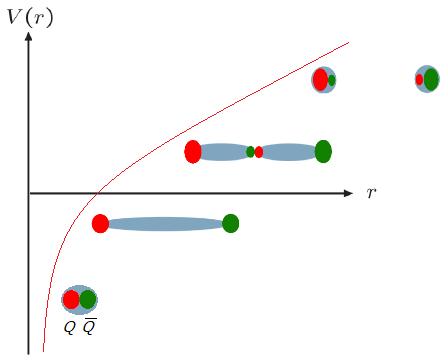
\includegraphics[width=9cm]{Potential.png}  
%Quelle: siehe Adrian BA und Mario MA
\caption{Verlauf des Quark-Antiquark-Potentials der QCD als Funktion des Abstands. Auf der Abbildung ist auch die Entwicklung der Hadronisierung durch Energiezufuhr dargestellt. In Anlehnung an \cite{krugermean2} und \cite{Chernodub:2010bi}.}
\label{Potential}
\end{figure}

\begin{figure}
\centering
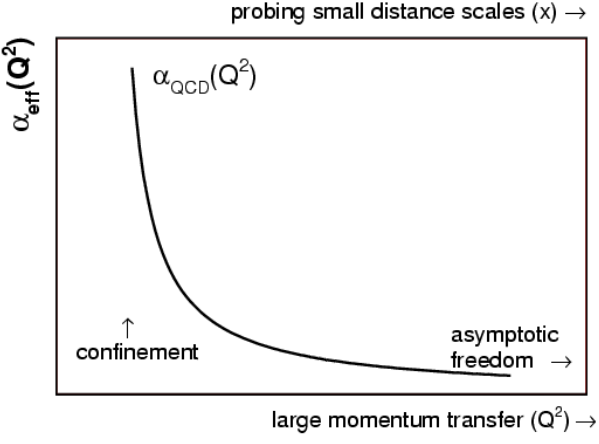
\includegraphics[width=9cm]{KoppKonst.png} 
%Quelle: http://home.thep.lu.se/~torbjorn/talks/durham09.pdf_modules
\caption{Kopplungskonstante der starken Wechselwirkung in Abhängigkeit des Abstands bzw. des Impulsübertrags. \cite{Group:2006bn}}
\label{KoppKonst}
\end{figure}
Es soll auch nicht unerwähnt bleiben, wie das Quark-Antiquark-Potential der QCD sich bei kleinen Abständen verhält. In diesem Fall dominiert der von $1/r$ abhängige Term und damit zeigt das Potential $V(r)$ ein Verhalten ähnlich dem wohlbekannten Coulomb-Potential. Außerdem enthält dieser Term die Kopplungskonstante der starken Wechselwirkung $\alpha_{\mathrm{s}}$, die sich als Funktion des Impulsübertrags $Q^{2}$ wie folgt darstellen lässt:
\begin{equation} \label{eq:KoppKonstante}
  \alpha_{\mathrm{s}}(Q^{2})\propto\dfrac{1}{\ln{\dfrac{Q^{2}}{\Lambda_{\mathrm{QCD}}^{2}}}}
\end{equation}
Dabei bezeichnet $\Lambda_{\mathrm{QCD}}$ den sogenannten Skalenparameter der QCD, bei dem $\alpha_{s}$ divergiert. Die Kopplungskonstante $\alpha_{\mathrm{s}}$ hängt im Gegensatz zur Kopplungskonstante der Quantenelektrodynamik (QED), der Theorie der elektromagnetischen Wechselwirkung, sehr stark vom Impulsübertrag $Q^{2}$ ab. Aufgrund dieses besonderen Merkmal, spricht man von der laufenden Kopplungskonstante (in Englisch: \textit{running coupling constant}). An dieser Stelle soll besonders betont werden, dass kleine Abstände gemäß den aus der De-Broglie-Wellenlänge gezogen Schlussfolgerungen große Impulsüberträge bedeuten. In diesem Zusammenhang ist zu beachten, dass $Q^{2}\propto 1/r$ gilt. Man beobachtet somit, dass die Kopplungskonstante und damit die Stärke der starken Wechselwirkung bei großen Impulsüberträgen bzw. bei kleinen Abständen abnimmt und gegen Null geht. Dieser bemerkenswerte Effekt wird asymptotische Freiheit genannt. Dies impliziert folgende physikalische Feststellung: Quarks verhalten sich bei sehr hohen Impulsüberträgen bzw. bei kleinen Abständen wie quasi-freie Teilchen. Ein solcher Zustand der Materie mit quasi-freien Quarks ist als Quark-Gluon-Plasma (QGP abgekürzt) bekannt.
\section{Quark-Gluon-Plasma}
\label{sec:QGP}
\begin{figure}
\centering
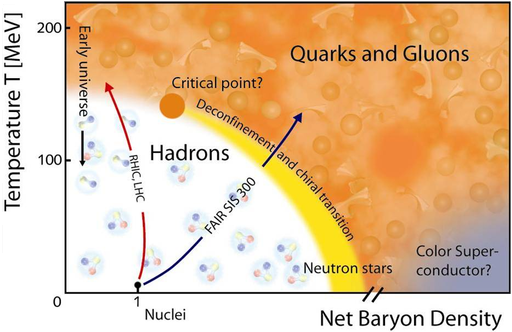
\includegraphics[width=13cm]{Phasenuebergang.png} 
%Quelle: suche sie in Google
\caption{Das Phasendiagramm der Materie. Die Phasen der Kernmaterie sind als Funktion sowohl der Temperatur als auch der Netto-Baryonen-Dichte dargestellt \cite{GSS}.}
\label{Phasenuebergang}
\end{figure}
Wie im letzten Kapitel erwähnt, können keine freien Quarks beobachtet werden. Allerdings vermutet man heute, dass sich das Universum während der ersten Augenblicke nach dem Urknall in einem Zustand befand, in dem Quarks aufgrund der hohen Temperaturen keine Hadronen bilden konnten und sich daher wie freie Teilchen verhielten. Dieser Zustand der Materie, in dem Quarks und Gluonen frei existieren ohne gebundene Zustände zu bilden, entspricht dem Quark-Gluon-Plasma \cite{sarkar2009physics}. \\
Um ein umfassendes Verständnis des QGP zu bekommen, kann der Phasenübergang von hadronischer Materie zum QGP untersucht werden. Abbildung \ref{Phasenuebergang} zeigt ein Phasendiagramm, das zwei unterschiedlichen Phasen der Kernmaterie in Abhängigkeit von zwei Zustandsgrößen, der Temperatur und der Netto-Baryonen-Dichte, darstellt. Die Netto-Baryonen-Dichte beschreibt die Anzahl von Baryonen minus die Anzahl von Antibaryonen pro Volumeneinheit \cite{buhrke2013geheimnisvoller}. Dazu ist anzumerken, dass die gelbe Kurve, die die jeweils in Weiß und in Orange gekennzeichneten Zustände voneinander abgrenzt, zurzeit nur vermutet werden kann. Nach unserem aktuellen Verständnis der Kernmaterie ist dann zu erwarten, dass man zum QGP bei sehr hohen Energiedichten kommen kann. Dies kann im Extremfall auf zwei Arten erreicht werden: entweder durch Erreichung einer hohen Temperatur oder bei sehr hohen Baryonen-Dichten. Im Folgenden werden nur diese zwei Fälle behandelt. Enorm hohe Temperaturen wie im frühen Universum führen zu hohen Energien, was sich in der Ausbildung des QGP niederschlägt. Demgegenüber befinden sich Baryonen bei einer hohen Dichte, äquivalent zu hohem Druck, so eng zusammen, dass sie sich überlappen, bis man sie nicht mehr voneinander unterscheiden kann. Aus diesem Phänomen entsteht ebenso ein QGP. In der Natur könnte sich ein Beispiel für dieses Szenario in den Zentren von Neutronensternen finden.\\
Angesichts dessen wird die Untersuchung des QGP sowie seiner Eigenschaften absolut notwendig, um unsere Erkenntnisse über die Struktur der Kernmaterie weiter zu vertiefen. Dafür muss man die Bedingungen zur Ausbildung eines QGP auf der Erde reproduzieren. Zu diesem Zweck setzt man sogenannte Schwerionenbeschleuniger, wie beispielsweise den LHC\footnote{\textit{englisch: Large Hadron Collider}}, ein. In einer solchen Anlage werden hochrelativisisch beschleunigte Schwerionen zur Kollision gebracht. Dadurch kann genügend Energie zur Erzeugung eines QGP bei einer niedrigen Netto-Baryonen-Dichte erreicht werden. Aus diesen ultrarelativistischen Schwerionenkollisionen entsteht eine breite Anzahl von Teilchen, die mit Hilfe von Detektoren entsprechend gemessen werden. Daraus lassen sich vielfältige Rückschlüsse über das QGP ziehen, die unseren Blick auf die Teilchenphysik vertiefen.
\section{Hadronenproduktion in Proton-Proton-Kollisionen}
\label{sec:Hadrprok}
\begin{figure}[H]
%Quelle: PhD_Phillip_Luettig
\centering
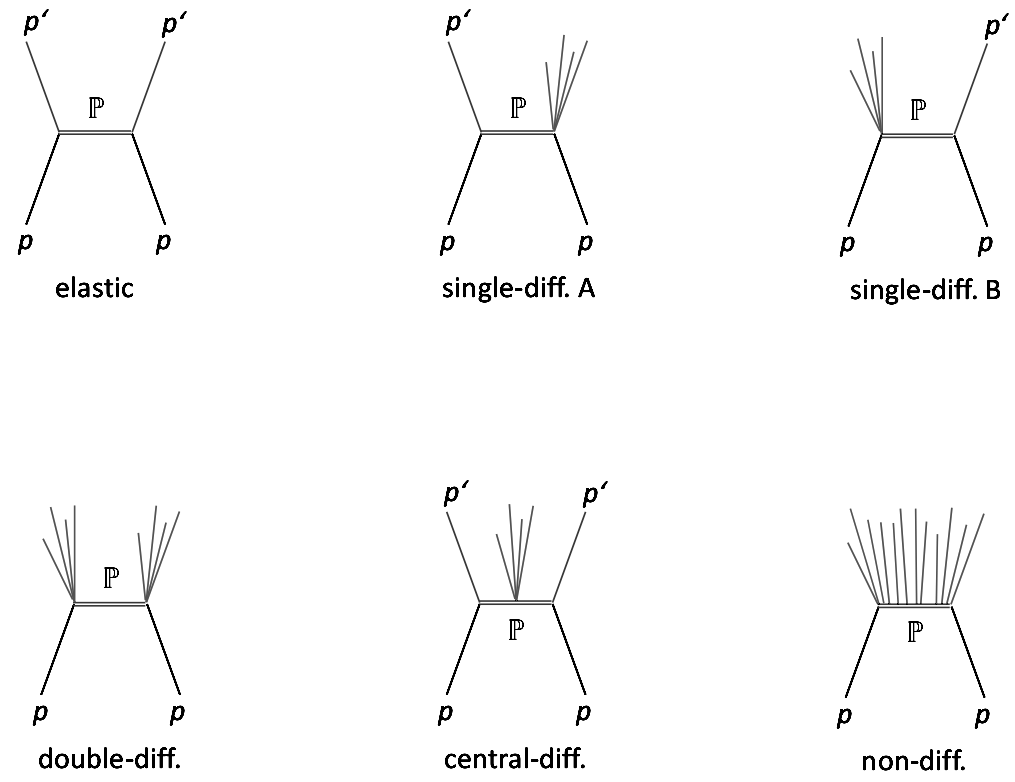
\includegraphics[width=13cm]{DiffractiveProzesse.png} 
\caption{Feynmann-Diagramme der möglichen Szenarien bei einer Proton-Proton-Kollision. Zeitachse hier von unten nach oben. Die durchgezogenen Linien, die in Zeitrichtung laufen, stellen den Verlauf der Protonen dar, während die Gruppierungen von Linien entstehende Teilchenstrahlen repräsentieren \cite{luttig2017charged}.}
\label{Diffractiv}
\end{figure}
In der vorliegenden Arbeit werden Messungen von Proton-Proton-Kollisionen unter der Annahme untersucht, dass dabei kein QGP entsteht. Die Messung dient als eine Referenzmessung zu Nukleus-Nukleus-Kollisionen, bei denen tatsächlich ein QGP erzeugt wird. Bei solchen Untersuchungen von stark wechselwirkender Materie besteht die Tendenz, Ereignisse, die zu unelastischen Streuprozessen gehören, zu selektieren. Der Grund dafür liegt darin, dass die kinetische Energie in solchen Kollisionen im Gegensatz zu elastischen Stößen nicht erhalten bleibt. Somit wird sich der Endzustand durch die Entstehung von einer Vielzahl neuer Teilchen aus\-zeichnen. Kollidierende Protonen müssen unelastisch wechselwirken, damit man eine Teilchenproduktion beobachtet.\\
Für eine nähere Erläuterung der Proton-Proton-Kollisionen, bei denen es zu Hadronenproduktion kommt, kann man alle möglichen Situationen untersuchen, die in einer unelastischen Streuung vorkommen können \cite{luttigMA2010}. Unelastische Prozesse unterteilen sich in zwei Gruppen in Abhängigkeit davon, ob die Protonen während des Prozesses eine Quantenzahl, wie z.B. die Farbladung, austauschen oder nicht. Gibt es tatsächlich einen Austausch von Quantenzahlen, dann spricht man von nicht-diffraktiven Kollisionen. Bei einer solchen Kollision zerfallen beide Protonen in eine breite Anzahl von Hadronen. Falls die Quantenzahlen hingegen keine Modifikation erfahren, bezeichnet man die Kollision als diffraktiv. Ferner klassifiziert man diffraktive Prozesse wie folgt:
\begin{itemize}
 \item Bei \textbf{einfach diffraktiven Prozessen} bleibt eines der Protonen bis auf die kinetische Energie unverändert, während das andere in mehrere Teilchen zerfällt.
 \item Bei \textbf{doppelt diffraktiven Prozessen} erfahren beide Protonen einen Zerfall. Allerdings fliegen die entstehenden Teilchenstrahlen anders als im Falle der nicht-diffraktiven Prozesse in gleicher Richtung wie die originalen Protonen.
 \item Bei \textbf{zentral diffraktiven Prozessen} sind die ursprünglichen Protonen zwar im Endzustand vorhanden, aber die jeweiligen kinetischen Energien wurden während des Stoßvorgangs modifiziert. Die von den Protonen verlorene kinetische Energie wandelt sich in einen Teilchenstrahl um.
\end{itemize}
Jeder dieser Prozesse ist durch eine bestimmte Geometrie charakterisiert, wie die Abbildung \ref{Diffractiv} zeigt. Unter Berücksichtigung aller genannten Faktoren stellen nicht-einfach diffraktive Wechselwirkungen, also doppelt und zentral diffraktive sowie nicht-diffraktive Prozesse, die relevantesten unelastischen Streuprozessen hinsichtlicht der Hadronenproduktion dar.\\
Gemäß des Impulsübertrags zweier kollidierenden Protonen lassen sich Streuprozesse ferner in harte und weiche Prozesse einteilen. Impulsüberträge erreichen bei harten Prozessen hohe Werte, während sie bei weichen Prozessen niedrig bleiben. Betrachtet man Formel \ref{eq:KoppKonstante}, dann stellt man fest, dass harte Prozesse eine kleine Kopplungskonstante $\alpha_\mathrm{s}$ aufweisen. Diese Tatsache erlaubt uns, harte Prozesse, an denen man aufgrund der hohen Hadronenproduktion interessiert ist, im Rahmen der Störungstheorie zu beschreiben. Solche Rechnungen sind als perturbative QCD (pQCD) bekannt.\\
An dieser Stelle soll zur Sprache gebracht werden, dass Protonen nicht nur aus drei einzelnen Quarks (\textit{uud}), den sogenannten Valenzquarks, bestehen, sondern sie eine Reihe von virtuellen Quark-Antiquark-Paaren, den Seequarks, bzw. Gluonen enthalten. Bei einer Proton-Proton-Kollision handelt sich damit um nichts anderes als einen Zusammenprall zwischen Valenzquarks, Seequarks und Gluonen, welche in diesem Zusammenhang als Partonen bezeichnet werden. \\
Nach all diesen Erwägungen und anhand pQCD kann man den differenziellen Wirkungsquerschnitt für die Hadronenproduktion, die in einer harten Proton-Proton-Kollision auftritt, durch einen Ausdruck definieren, der in drei unabhängige Faktoren unterteilt ist: die \textit{Parton Distribution Function} $\mathrm{PDF}$, der elementare
Wirkungsquerschnitt $\sigma$ und die Fragmentationsfunktion $\mathrm{D}$:
\begin{equation}
 \sigma_{\mathrm{pp}} = \mathrm{PDF}(x_1, Q^2) \otimes \mathrm{PDF}(x_2, Q^2) \otimes \sigma(x_1, x_2, Q^2) \otimes \mathrm{D}(z_\mathrm{h}, Q^2) 
\end{equation}
Diese Rechenoperation wird Faktorisierung genannt \cite{Collins:1989gx}. Dabei bezeichnet die \textit{Parton Distribution Function} $\mathrm{PDF}(x_i, Q^2)$ die Dichteverteilung eines Partons, das einen bestimmten Impulsübertrag $Q^2$ und einen Anteil des Gesamtimpuls des Hadrons $x = p_{\mathrm{Parton}}/p_{\mathrm{Hadron}}$ besitzt. Andererseits beschreibt der elementare Wirkungsquerschnitt $\sigma$ die Wahrscheinlichkeit, mit der zwei Protonen gemäß der pQCD kollidieren können. Letztendlich gibt die Fragmentationsfunktion die Wahrscheinlichkeit an, dass der Endzustand einer Kollision aus einem gegebenen Quark oder Gluon stammt, und sie beschreibt damit die Teilchenproduktion dieses Endzustands.\\
Zur Untersuchung von Stoßvorgängen berücksichtigt man ferner den zur Strahlachse senkrecht stehenden Impulsanteil, den Transversalimpuls $p_{\mathrm{T}}$. Dieser transversale Impulsanteil kann nur durch eine Kollision zweier Teilchen entstehen. Andernfalls besitzen Teilchen auf Grund der Beschleunigung im LHC nur einen longitudinalen Impulsanteil. Die genannte Faktorisierung ist in der Lage, die Teilchenproduktion nur für große Transversalimpulse zu beschreiben. Für kleine Transversalimpulse, in denen weiche Prozesse die größte Rolle spielen, benötigt man hingegen phänomenologische Modelle.\\
Neben diesen Betrachtungen stellt die Gesamtenergie der Protonen, die kollidieren, eine entscheidende Größe bei der Betrachtung von Streuprozessen dar. Sie ergibt sich im Falle eines Experiments mit kollidierenden Teilchenstrahlen aus der Addition der Ruheenergie und der kinetischen Energie der Teilchen. In der Teilchenphysik be\-zeichnet man sie als Schwerpunktsenergie $\sqrt{s}$.\\
Zur Analyse von Hadronenproduktionen in Proton-Proton-Kollisionen untersucht man häufig die Anzahl erzeugter Teilchen als Funktion des Transversalimpulses. Zu diesem Zweck besteht die allgemeine Strategie der vorliegenden Arbeit darin, die  $p_{\mathrm{T}}$-Verteilung der in Proton-Proton-Kollisionen erzeugten Teilchen zu berechnen. Wegen der Eigenschaften der für die Vermessung der generierten Teilchen angewendeten Detektoren, auf die im Kapitel \ref{cha:EAufbau} ausführlich eingegangen wird, können elektrisch geladene Teilchen besonders präzise aufgezeichnet werden. Im Hinblick auf die durchgeführte Analyse genügen solche Teilchen, um das Verhalten der restlichen Teilchen zu beschreiben. Daher wird konkret die $p_{\mathrm{T}}$-Verteilung geladener Teilchen evaluiert, die in Proton-Proton-Kollisionen erzeugt werden.
\section{Monte-Carlo-Simulationen}
\label{sec:MC}
Die gemessenen Daten einer hochenergetischen Kollision werden durch die begrenzte Effizienz der Detektoren beeinflusst. Dadurch tritt eine Abweichung dieser Messdaten von den tatsächlichen Daten auf, was dazu zwingt, Korrekturen anhand computergestützten Simulationen anzuwenden. Diese Simulationen müssen in der Lage sein, die identischen Bedingungen des Experiments zu reproduzieren und die daraus resultierenden Ergebnisse zu verarbeiten. Diese Situation wirft allerdings folgendes Problem auf: die erwähnten Simulationen sollen sich exakt an die vom QCD vorgeschlagenen Modellen anpassen, die analytisch nicht gelöst werden können oder die aufwendigen numerischen Lösungen fordern. Aus diesem Grund verwendet man zur Erzeugung der Simulationen eine probabilistische und hocheffektive Methode, die sogenannte Monte-Carlo-Studie (MC-Studie abgekürzt)\cite{PHUHN15}.\\ 
Die Monte-Carlo-Studie basiert auf der Beobachtung, dass die relative Häufigkeit eines Zufallsergebnisses an seine theoretische Wahrscheinlichkeit annähert, wenn man das zugrundeliegende Zufallsexperiment oft genug unter denselben Bedingungen wiederholt. In der Teilchenphysik lassen sich Teilchenkollisionen mithilfe einer computergestützten Monte-Carlo-Studie gemäß der QCD nachbilden. Anschließend werden entsprechend Zufallswerte ausreichend häufig erzeugt, um das Verhalten der aus der Kollision resultierenden Teilchen zu ermitteln, wie z.B. die eingeschlagenen Zerfallsketten oder die kinematischen Eigenschaften der Teilchen. Es sei jedoch vermerkt, dass man am Ende kein eindeutiges Ergebnis erhält, sondern eine Wahrscheinlichkeitsverteilung. Solche Monte-Carlo-Studien, die für die Beschreibung von Prozesse in der QCD gebraucht werden, sind als Monte-Carlo-Simulationen bekannt.\\
%WICHTIG: zu korrigieren: GEANT3->Detector, PYTHIA6->Event Genarator
In der Hochenergiephysik werden Programme, die Monte-Carlo-Simulationen durchführen, als Monte-Carlo-Generatoren bezeichnet. Im vorliegenden Fall wird der Monte-Carlo-Generator PYTHIA, um in Kollisionen erzeugte Teilchen zu simulieren. Ferner wird zur Korrektur der Messdaten der Monte-Carlo-Generator GEANT3\footnote{englisch: \textit{\textbf{GE}ometry \textbf{AN}d \textbf{T}racking}} verwendet, welcher den Durchgang dieser erzeugten Teilchen durch Detektoren simuliert. GEANT3 besitzt im Unterschied zu anderen Monte-Carlo-Generatoren die Fähigkeit, das Ansprechverhalten der Detektoren zu beschreiben. 
%https://arxiv.org/pdf/0710.3820.pdf
\chapter{Experimenteller Aufbau}
\label{cha:EAufbau}
Die erwähnten experimentellen Messungen und damit die Forschung der Struktur der Materie werden in Europa durch die Europäische Organisation für Kernforschung (CERN\footnote{französisch: \textit{\textbf{C}onseil \textbf{E}uropéen pour la \textbf{R}echerche \textbf{N}ucléaire}} abgekürzt) durchgeführt. Dieses Projekt hat seinen Sitz in Genf und entwickelt sich derzeit dank der Beteiligung von 22 europäischen Mitgliedstaaten. Im Rahmen dieser Zusammenarbeit sind vier große Experimente entstanden: ATLAS\footnote{englisch: \textit{\textbf{A} \textbf{T}oroidal \textbf{L}HC \textbf{A}pparatu\textbf{S}}}, CMS\footnote{\textit{\textbf{C}ompact \textbf{M}uon \textbf{S}olenoid}}, ALICE\footnote{\textit{\textbf{A} \textbf{L}arge \textbf{I}on \textbf{C}ollider \textbf{E}xperiment}} und LHCb\footnote{\textit{\textbf{L}arge \textbf{H}adron \textbf{C}ollider \textbf{b}eauty}}. Das CERN beherbergt den größten Teilchenbeschleuniger der Welt, den LHC, und wird somit weltweit führend bei der wissenschaftlichen Recherche.  
\section{LHC}
\label{sec:LHC}
Im Jahr 2008 wurde der zur Zeit leistungsstärkste Teilchenbeschleuniger LHC erstmals in Betrieb gesetzt. Diese ringförmige Einrichtung, deren Umfang $26.7$ km beträgt, gehört zum Typ Synchrotron und ist daher in der Lage, zwei beschleunigte Teilchenstrahlen auf kreisförmige Bahnen zu halten. Die Teilchenstrahlen erreichen annähernd Lichtgeschwindigkeit und bewegen sich in entgegengesetzter Richtung durch Ultrahochvakuum, bis sie kollidieren. Damit sie die festgelegten Kreisbahnen perfekt beschreiben, verwendet man supraleitende Elektromagnete, die über ständige Helium-Versorgung zur Abkühlung auf eine Temperatur kleiner als $2$ K verfügen \cite{CernWebpage}.\\
Im LHC werden zurzeit drei Arten von Kollisionen durchgeführt: Blei-Blei, Proton-Proton und Proton-Blei-Kollisionen. Die Schwerpunktsenergie $\sqrt{s}$ einer solchen Kollision wird durch die Energie der beteiligten Hadronenstrahlen $E$ bestimmt:
\begin{equation}
\sqrt{s}=2E
\end{equation} 
Die bisher maximal erreichte Schwerpunktsenergie in Proton-Proton-Kollisionen beträgt zurzeit $\sqrt{s} = 13$ $\mathrm{TeV}$ \cite{Bruning:782076}. \\
Die entgegengesetzt beschleunigten Teilchenstrahlen kreuzen sich an vier festgelegten Stellen des LHC-Tunnels. An jedem dieser Punkte befindet sich eines der vier großen Experimente des LHC. Da die in dieser Arbeit vorgestellte Analyse auf vom ALICE-Experiment erfassten Daten basiert, wird dieses Experiment im Folgenden detaillierter behandelt.
\section{ALICE}
\label{sec:ALICE}
Das ALICE-Experiment fokussiert seine Tätigkeit darauf, stark wechselwirkende Materie mittels der erwähnten Teilchenkollisionen zu untersuchen. Das Ziel besteht darin, ein umfassendes Verständnis des QGP zu erlangen. Das ALICE-Detektorsystem mit den Abmessungen $16$ $\mathrm{x}$ $16$ $\mathrm{x}$ $25$ $\mathrm{m^3}$ ist aus 18 Detektoren aufgebaut, welche die vielfältigen Aufgaben übernehmen, für die das Experiment entwickelt wurde. Zu den Aufgaben gehören beispielsweise die Rekonstruktion der Teilchenspuren, die Identifizierung dieser Teilchen, die Vermessung der im Detektormaterial deponierten Energie der Teilchen und die Bestimmung der Kollisionspunkte \cite{breskin2009cern}.\\
Das ALICE-Detektorsystem lässt sich in drei Bestandteile mit unterschiedlichen Funktionen unterteilen: einen zylindersymmetrischen Aufbau, der die Strahlachse umgibt, verschiedene Vorwärts-Detektoren, die unter anderem zur Bestimmung der Zentralität der Blei-Blei-Kollisionen dienen, und einen Myonenarm, der auf die Messung von Myonen spezialisiert ist. Da die in dieser Analyse verwendeten Messdaten aus Messungen mit dem zylindrischen Teil stammen, wird insbesondere auf die Detektoren eingegangen, aus denen dieser Teil besteht. In der Abbildung \ref{AliceDetector} ist der schematische Aufbau des ALICE-Detektors dargestellt.\\
Im zylindersymmetrischen Element des ALICE-Detektorsystems unterscheidet man sechs Detektoren. Die Detektoren sind durch einen solenoiden Magnet, der L3 Magnet, umgeschlossen, der für die Erzeugung eines Magnetfeldes von $B = 0.5$ T verantwortlich ist. Dieses Magnetfeld verursacht die Krümmung der Trajektorie geladener Teilchen. Dadurch lässt sich der Impuls der Teilchen bestimmen. Die für diese Arbeit relevantesten Detektoren heißen \textit{Inner Tracking System} und \textit{Time Projection Chamber} (jeweils ITS und TPC abgekürzt). Das ITS befindet sich an dem innersten Punkt des ALICE-Detektors und umgibt die Strahlachse. Nach außen gehend liegt die TPC am nächsten. Wegen ihrer großen Relevanz für die Arbeit wird nachfolgend auf Details der Detektoren ITS und TPC eingegangen.\\
An den beiden Enden des ITS ist der V0-Detektor, einer der Vorwärts-Detektoren, zu finden. Dieser Detektor dient zur Bestimmung der Zentralität bei Schwerionenkollisionen. Außerdem wird dafür verwendet, die Kollisionen nach den im Abschnitt \ref{sec:Hadrprok} beschriebenen Kriterien zu evaluieren und sie zwischen den verschiedenen Gruppen von Streuprozessen zu unterscheiden. Der V0 ist aus zwei Subdetektoren, dem V0C und dem V0A, aufgebaut, die nach dem Funktionsprinzip von Szintillatordetektoren betrieben werden. Sie befinden sich jeweils $0.9$ m und $3.4$ m vom primären Kollisionsvertex entfernt. 
\begin{figure}
\centering
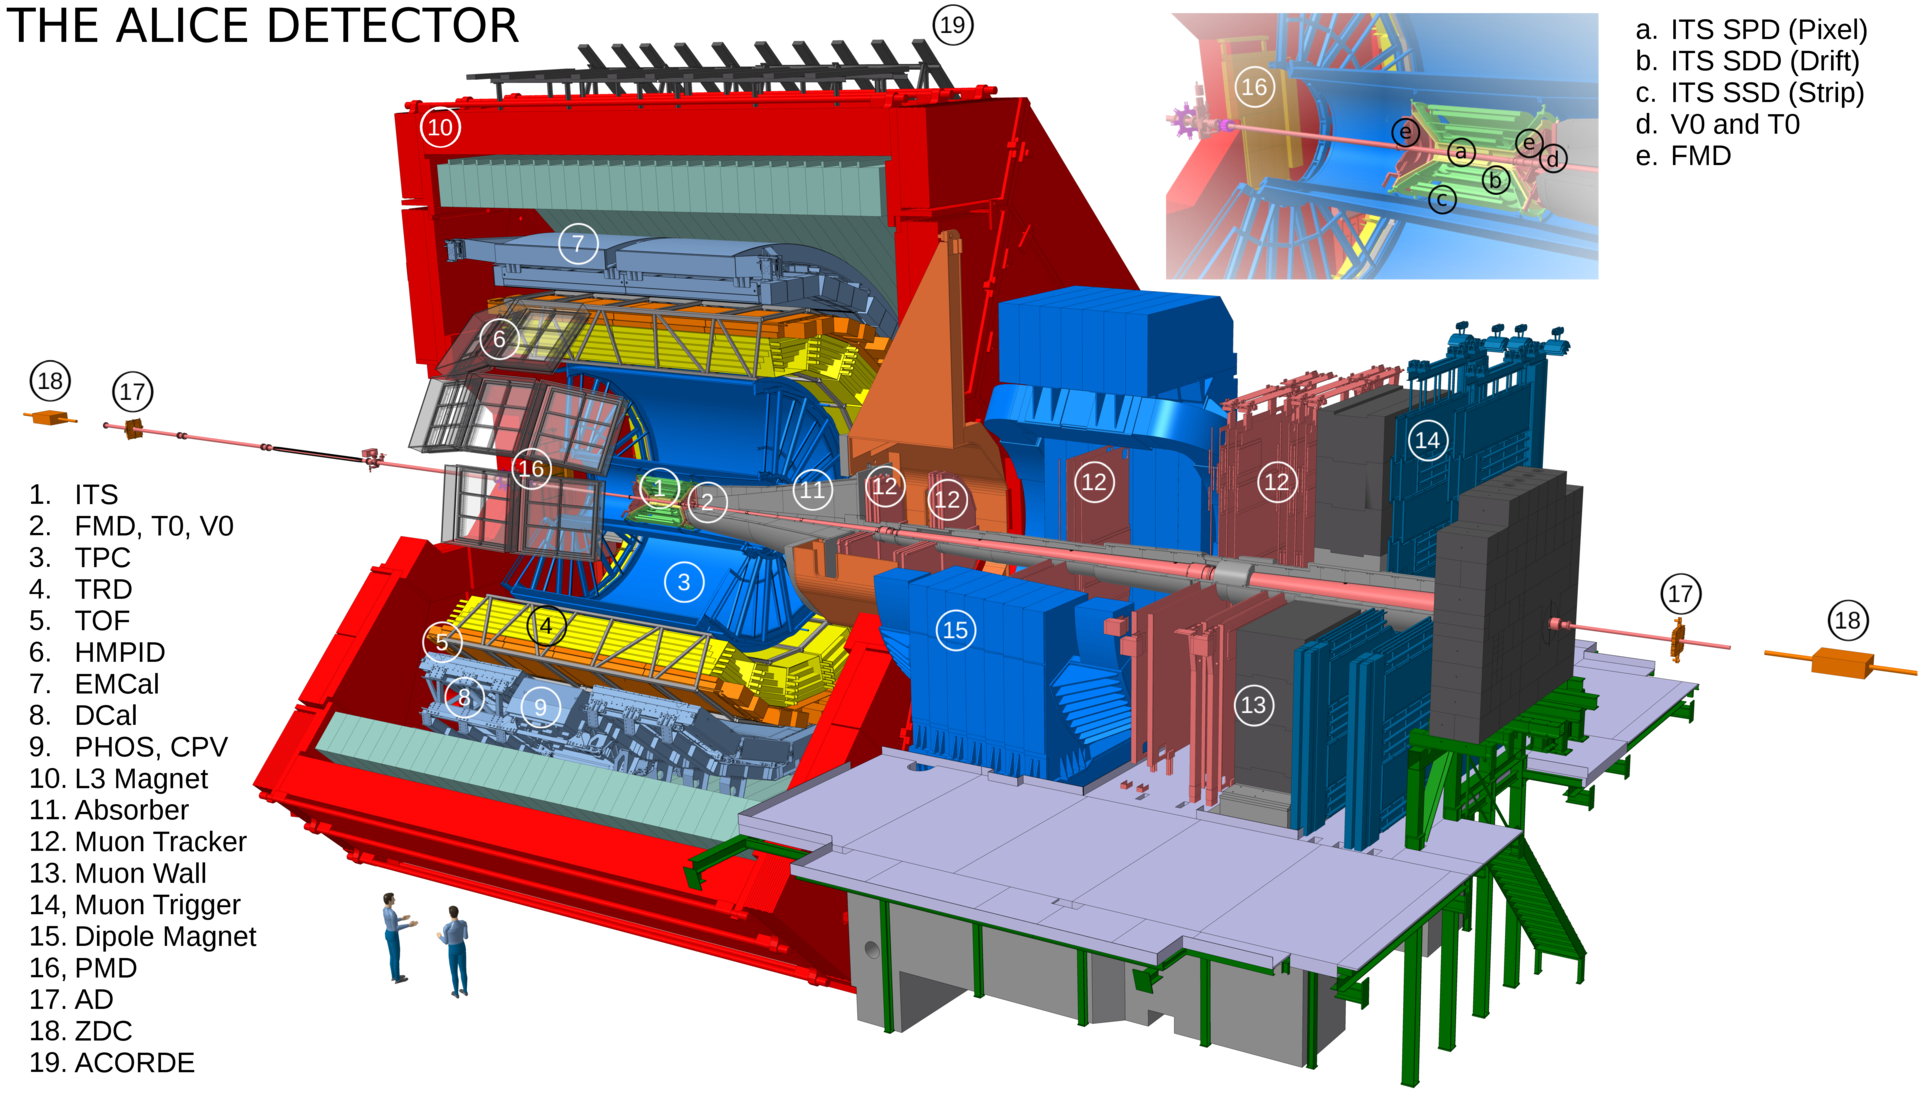
\includegraphics[width=15cm]{Alice.png} 
\caption{Schematische Darstellung des ALICE-Detektors \cite{Tauro:2263642}.}
\label{AliceDetector}
\end{figure}
\subsection{Inner Tracking System}
Das ITS ermöglicht die Rekonstruktion des primären Kollisionsvertex sowie die Messung der Teilchenspuren. Außerdem wird es zur Teilchenidentifizierung verwendet. Das ITS erlaubt ferner, über eine bessere Auflösung zu verfügen und damit die Vermessung des Transversalimpulses zu verbessern. Es soll jedoch betont werden, dass sich die Aufgaben des ITS nicht darauf beschränken, sondern es zu allen Bereichen des ALICE-Experiments beiträgt.\\
Dieser zylinderförmige Detektor, der einen gesamten Radius von $51$ cm besitzt, besteht wiederum aus drei Subdetektoren mit jeweils zwei Schichten aus Silizium, also aus Halbleitermaterial. Die Schichten befinden sich in radialen Abständen zwischen $3.9$ cm und $43$ cm von der Strahlachse. Die Subdetektoren sind in radialer Richtung wie folgt angeordnet: 
\begin{itemize}
\item \textit{Silicon Pixel Detector} (SPD)\\
Die zwei innersten Schichten des ITS bilden den Subdetektor SPD, welcher sich hauptsächlich der Bestimmung der Kollisionspunkte widmet. Der SPD wurde speziell für ein Umfeld konzipiert, in dem nach einer Kollision eine hohe Spurdichte und Radioaktivität dominieren. Zur Messung generierter Teilchen wird berücksichtigt, dass geladene Teilchen, die durch Halbleitermaterial fliegen, freie Ladungsträger erzeugen. Solche Ladungsträger wandern dann zu Elektroden aus Metall. Der resultierende Stromsignal kann in den Transversalimpuls der Teilchen umgerechnet werden. 
\item \textit{Silicon Drift Detector} (SDD)\\
Der SDD besteht aus den mittleren Schichten des ITS und handelt sich um einen Driftdetektor. Im Unterschied zum SPD driften die freigesetzten Ladungsträger, die in der Mitte des Detektors liegen, aufgrund der angelegten Spannung zu den Ränder des SDD. Der Detektor ist mit verschiedenen Ausleseanoden ausgestattet, die die Spuren dadurch messen können. Dieser Aufbau erhöht die Anzahl von messbaren Spuren im Vergleich zum SPD. Außerdem helfen die SDD-Schichten dabei, den spezifischen Energieverlust $\mathrm{d}E/\mathrm{d}x$ der Teilchen durch das Detektormaterial zu bestimmen. Diese Größe ist direkt mit der Ladung und der Energie der Teilchen verbunden und erlaubt somit ihre Identifizierung. Mehr Details über den spezifischen Energieverlust werden später diskutiert.
\item \textit{Silicon Strip Detector} (SSD)\\
Der äußerste Subdetektor des ITS wurde möglichst nah an die TPC platziert, damit der Übergang der Teilchen zu dieser Kammer die Spurrekonstruktion nicht beeinträchtigt. Der SSD ist in der Lage, eine zweidimensionale Aufzeichnung der Flugbahn geladener Teilchen durchzuführen. Erzeugte Teilchen werden in ähnlicher Weise wie beim SPD gemessen. Der SSD sammelt ebenfalls Daten, um den spezifischen Energieverlust der Teilchen auszurechnen. 
\end{itemize}

\subsection{Time Projection Chamber}
Die TPC stellt den wichtigsten Detektor des zylindersymmetrischen Elements vom ALICE dar und sorgt neben den restlichen zentralen Detektoren für die Messung des Transversalimpulses der erzeugten geladenen Teilchen sowie für die Spurrekonstruktion. Darüber hinaus wird sie zur Identifikation der Teilchen und zur Bestimmungs der Kollisionsvertices eingesetzt.\\
Die Innen- und Außenradien der TPC messen jeweils $0.85$ cm und $2.5$ m, während die Länge des Detektors $5$ m beträgt. Das Innere dieser Spurendriftkammer ist mit einem Gasgemisch aus Neon, Kohlendioxid und Stickstoff gefüllt. Diese Mischung, die ein Volumen von $88$ $\mathrm{m^3}$ besetzt, dient als Detektormedium und steht unter elektrischer Spannung. Dies erlaubt erzeugten geladenen Teilchen, Atomkerne zu ionisieren. Diese fliegen dann zur sich in der Mitte der Spurendriftkammer befindenden Elektroden. Durch die Ionisation werden Ladungsträger frei, die zu den Ausleseelektroden an den Endkappen des Detektors driften. Die resultierenden Signale werden dann für die Rekonstruktion der Spur verwendet.\\
\begin{figure}[tb!]
\centering
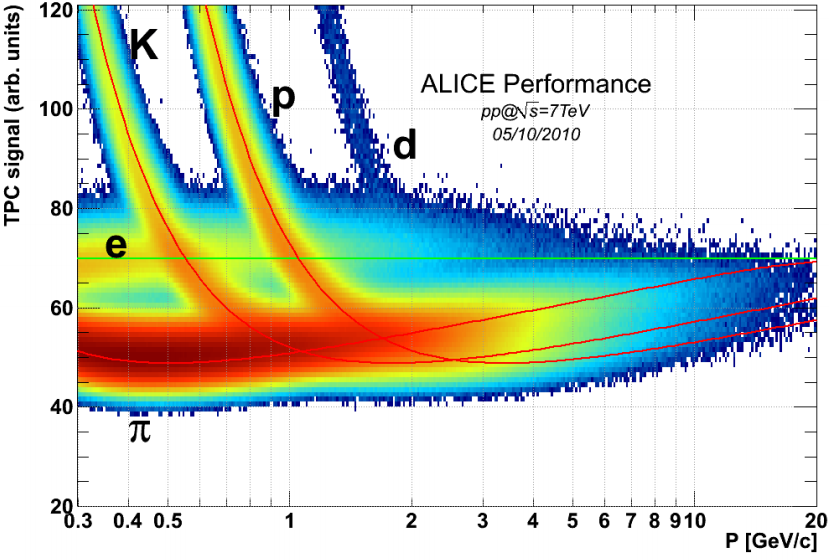
\includegraphics[width=13cm]{EnergieverlustTPC.png} 
\caption{Aufnahme des spezifischen Energieverlust der geladenen Teilchen Kaon $K$, Proton $p$, \textit{down}-Quark $d$ und Elektron $e$ als Funktion des Impulses in der TPC \cite{PHUHN17}.}
\label{EnergieverlustTPC}
\end{figure}
\hspace{-0.206cm}Das elektrische Signal, das ein ankommender Ladungsträger generiert, zeigt eine Abhängigkeit von der Energie des Ladungsträgers. Daraus lässt sich die Energie bestimmen, die das ursprüngliche fliegende Teilchen aufgrund der erfahrenen Stöße und der Ionisation von Atomkernen verliert. Sie wird als spezifischen Energieverlust bezeichnet und lässt sich mit der sogenannten Bethe-Formel im Mittel beschrieben:
\begin{equation}
- \left<\frac{\mathrm{d}E}{\mathrm{d}x}\right> = \frac{4 \pi n z^2}{m_e c^2 \beta^2} \cdot \left(\frac{e^2}{4 \pi \epsilon_0}\right)^2 \left[ \ln{\frac{2 m_e c^2 \beta^2}{I \cdot (1 - \beta^2)}} - \beta^2 \right] 
\end{equation}
Dabei symbolisiert $E$ die Energie des Teilchens, $x$ die zurückgelegte Strecke im Medium mit der Elektronendichte $n$ und dem mittleren Anregungspotential $I$, $z$ die Ladung des Teilchens, $e$ die Elementarladung, $v$ die Geschwindigkeit des Teilchens, $\beta$ der Anteil dieser Geschwindigkeit zur Lichtgeschwindigkeit, $\epsilon_0$ die elektrische Feldkonstante und $m_e$ die Ruhemasse des Elektrons. Abbildung \ref{EnergieverlustTPC} zeigt den spezifischen Energieverlust von geladenen Teilchen in Abhängigkeit des Impulses.\\
Diese Größe zusammen mit der messbaren Zeitspanne der Drift des Teilchens bieten die Möglichkeit an, das Teilchen zu identifizieren. Allerdings sieht man in der Abbildung, dass sich die Teilchensorten ab einem bestimmten Impuls sehr schwierig voneinander unterscheiden lassen. Andere zentrale Detektoren, wie der \textit{Transition Radiation Detector} (TRD), der \textit{Time of Fligt} (TOF) oder der \textit{High-Momentum Particle Identification Detector} (HMPID) werden daher zusätzlich zur TPC für die Teilchenidentifikation verwendet.
 
\chapter{Analyse}
\label{cha:Analyse}
Diese Arbeit untersucht Proton-Proton-Kollisionen bei einer Schwerpunktsenergie von $\sqrt{s} = 5.02$ $\mathrm{TeV}$, die mit dem ALICE-Detektor gemessen wurden. Dabei werden hier die erzeugten geladenen Teilchen betrachtet. Die gemessenen Daten werden anschließend verarbeitet, um eine Verteilung des Transversalimpulses oder $p_{\mathrm{T}}$-Spektrum zu erhalten. Das $p_{\mathrm{T}}$-Spektrum wird dann mit Ergebnissen, die anhand von MC-Simulationen gewonnen wurden, verglichen und durch Verwendung verschiedener Strategien, die im folgenden Abschnitt ausführlich dargestellt werden, entsprechend korrigiert. Schließlich werden systematische Unsicherheiten auf das korrigierte $p_{\mathrm{T}}$-Spektrum abgeschätzt, die durch die vorgestellte Analyse verursacht werden.
\section{Datenauswahl}
In dieser Arbeit werden gemessene Daten, die aus im Jahr 2017 gemessenen Proton-Proton-Kollisionen stammen, betrachtet. Die gemessenen Daten unterteilen sich in zwei Datenmengen in Abhängigkeit davon, ob die Kollisionen mithilfe der SDD-Schichten des ITS rekonstruiert wurden oder nicht. Ob der SDD zur Rekonstruktion verwendet wird oder nicht, liegt an folgendem Phänomen dieses Teilchendetektors: Nachdem ein Teilchen mit diesem Detektor gemessen wird, vergeht aufgrund technischer Merkmale eine gewisse Zeitspanne, während der kein weiteres Teilchen nachgewiesen werden kann. Diese Zeitspanne nennt man Totzeit. Für die SDD-Schichten dauert sie im Vergleich zum restlichen Detektor sehr lang. Dies führt dazu, dass man durch Verzicht auf den Einsatz der SDD-Schichten viel Zeit spart und dadurch mehr Kollisionen messen kann. Allerdings verringert sich dabei die Präzision der Bestimmung des Kollisionspunktes. Die Datenmenge, die die ohne SDD-Schichten rekonstruierten Ereignisse enthält, benennt man \textit{FAST}. Andererseits wird die Datenmenge, die aus den mit SDD gemessenen Ereignissen besteht, als \textit{CENT} bezeichnet. Zusätzlich kann man die Ereignisse des CENT-Datensatzes ohne die Verwendung des SDD-Detektors rekonstruieren. Diese Tatsache erleichtert den Vergleich zwischen den mit und den ohne SDD rekonstruierten Ereignissen. In der Tabelle \ref{tab:CENTundFAST} kann man die Anzahl von Ereignissen der jeweiligen Datenmengen betrachten. In diesem Zusammenhang ist darauf hinzuweisen, dass diese Ereignisse ein konkretes Auswahlverfahren, welches im nächsten Abschnitt näher erläutert wird, durchgelaufen haben. \\
Die Verwendbarkeit der größten Anzahl von Ereignissen würde erlauben, über das statistisch präzisere Ergebnis zu verfügen. Im vorliegenden Fall beinhaltet der \textit{FAST}-Datensatz fast doppelt so viele Ereignisse wie der \textit{CENT}-Datensatz. Um auf beide Datenmengen zurückgreifen zu können, soll allerdings zuallererst untersucht werden, wie sich die Abwesenheit der SDD-Schichten bei der Messung der Kollisionen auf die Ergebnisse auswirkt. Für die Durchführung dieser Studie werden zuerst die unkorrigierten $p_{\mathrm{T}}$-Spektren, die aus den verschiedenen  Datenmengen resultieren, miteinander verglichen. Darüber hinaus wird ein Vergleich der jeweiligen relativen $p_{\mathrm{T}}$-Auflösungen angestellt, um mehr Auskunft über den Einfluss des Einsatzes der SDD-Schichten auf die gemessenen Daten zu erhalten. Diese Elemente werden feststellen, ob die \textit{FAST}-Ereignisse und die ohne SDD rekonstruierten \textit{CENT}-Ereignisse kombiniert werden dürfen. In diesem Fall könnte man über die maximale Anzahl von Ereignissen verfügen.
\begin{table}
\centering
\begin{tabular}{|c|c|c|c|}
\hline
\multicolumn{1}{|c}{\textbf{Datenmenge}} & \multicolumn{1}{|c|}{\textbf{FAST}} & \multicolumn{2}{c|}{\textbf{CENT}} \\
\cline{3-4}
 &  & \textbf{mit SDD} & \textbf{ohne SDD} \\
\hline
\hline
$N_{E}$ in Mio. & $700$ & $401$ & $395$ \\ 
%\cline{2-5}
\hline
\end{tabular}
\caption{Anzahl von Ereignissen $N_{E}$ der jeweiligen Datenmengen. Die Anzahl von Ereignissen von CENT mit SDD ist nicht gleich der von CENT ohne SDD, obwohl es sich um die selben Ereignisse handelt. Da die verwendete Selektion der Ereignisse und damit $N_{E}$ durch die Abwesenheit der SDD-Schichten beeinflusst werden, tritt eine Abweichung auf.}
\label{tab:CENTundFAST}
\end{table} 

\section{Auswahlkriterien}
\subsection{Selektion der Ereignisse}
\begin{figure}
\centering
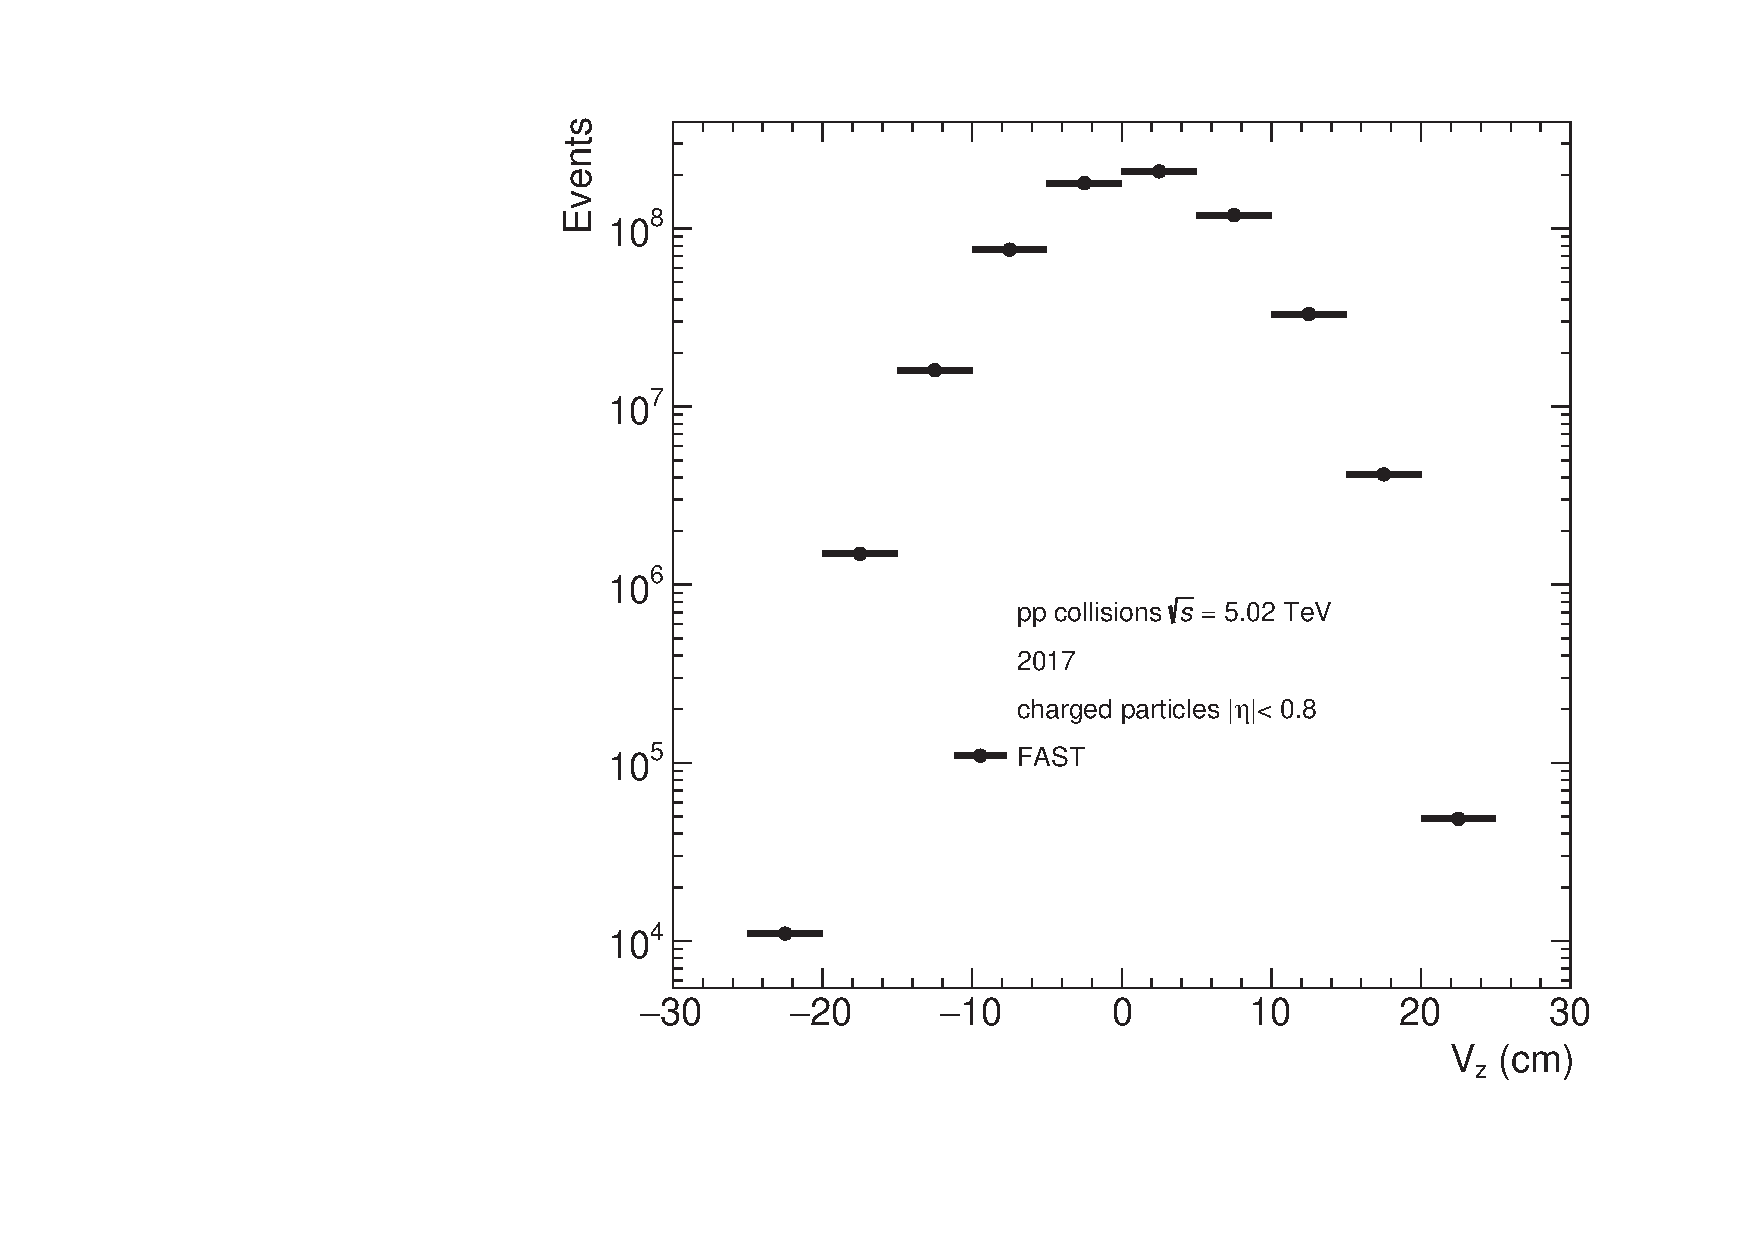
\includegraphics[width=11cm]{Plots/VertexZFAST.pdf} 
\caption{Verteilung der Ereignisse als Funktion der Position des Kollisionsvertex entlang der Strahlachse.}
\label{VertexZ}
\end{figure}
Im ALICE-Experiment erforscht man stark wechselwirkende Materie. Die zu untersuchenden Ereignisse müssen daher aus unelastischen Streuprozessen stammen, wie bereits ausführlich diskutiert. Um experimentell nachweisen zu können, ob eine unelastische Kollision stattgefunden hat, bedarf es einer technischen Methode. Eine solche Methode wird als Trigger bezeichnet. In dieser Arbeit wird dafür eine Kombination der Signale der Detektoren SPD und V0 verwendet. Dadurch kann gewährleistet werden, dass bei einer Messung, mit hoher Wahrscheinlichkeit tatsächlich eine unelastische Kollision stattgefunden hat, ohne durch die Messung die eigentliche Produktion der neuen Teilchen zu verändern. Dieser Trigger wird dann als \textit{minimum bias} (in Deutsch: kleinster Einfluss) Trigger bezeichnet. \textit{Minimum bias} selektiert im Vergleich zu anderen möglichen Konfigurationen des Triggers am meisten Ereignisse. In der in dieser Arbeit vorgenommenen Studie wird \textit{minimum bias} zur Selektion der gemessenen Ereignisse benutzt.\\ 
Außerdem ist der Trigger so konfiguriert, dass er unelastische Stöße auswählt, in denen die Hadronenproduktion maximal wird. Der für diese Arbeit angewendete Trigger wird unter Berücksichtigung dieser Eigenschaften so optimiert, dass er für nicht-einfach diffraktive Wechselwirkungen Vorrang einräumt.\\
Für die vorliegende Untersuchung wird zusätzlich gefordert, dass die Kollisionsvertices der Ereignisse $V_{Z}$ innerhalb $\pm 10$ cm Abstand vom Nominalvertex, also von $V_{Z} = 0$ cm, entlang der Stahlachse liegen. Abbildung \ref{VertexZ} zeigt zur Veranschaulichung die Verteilung der aus \textit{FAST} stammenden Ereignisse in Abhängigkeit der Position des Kollisionsvertex $V_{Z}$.
\subsection{Spurselektion}
\label{sec:Spurselektion}
In der experimentellen Teilchenphysik drückt man den Winkel $\theta$ zwischen der Flugrichtung eines erzeugten Teilchens und der Strahlachse durch die sogenannte Pseudorapidität $\eta$ aus, die folgendermaßen im Zusammenhang mit dem erwähnten Winkel steht:
\begin{equation}
 \eta = -\ln{\tan{\dfrac{\theta}{2}}}
\end{equation}
Um eine möglichst hohe Qualität der Daten zu selektieren, werden in dieser Arbeit die geometrischen Anforderungen so gewählt, dass der Polarwinkel $\theta$ mit der geometrischen Abdeckung der Detektoren TPC und ITS übereinstimmt. Daher fordert man, dass sich die Pseudorapidität der gemessenen Teilchen im Intervall $|\eta| < 0.8$ befindet.\\
Im Rahmen dieser Arbeit werden weitere Auswahlkriterien für die Spuren der Teilchen mit dem Ziel angewendet, die physikalisch relevanten Daten zu selektieren. Dabei sollte betont werden, dass nur elektrisch geladene Teilchen eine verfolgbare Spur hinterlassen können.\\
Teilchen, die entweder aus der Kollision oder aus Zerfällen entstehen, die in unmittelbarer Nähe des Kollisionsvertex vorkommen, und eine Lebensdauer \hspace{2cm} $\tau > 1$ cm/\textit{c} besitzen, nennt man im ALICE-Experiment Primärteilchen \cite{ALICE-PUBLIC-2017-005}. Diese Definition von Primärteilchen bezieht folgende Teilchen in Reihenfolge der Häufigkeit ein: Pion $\pi^+$, Kaon $K^+$, Proton $p$, die Sigma-Baryonen $\Sigma^+$ und $\Sigma^-$, Elektron $e^-$, Muon $\mu^-$, Xi-Baryon $\Xi^-$ und Omega-Baryon $\Omega^-$ sowie deren entsprechenden Antiteilchen.\\ 
Im Wesentlichen bestehen die erwähnten Auswahlkriterien darin, die gemessenen Teilchenspuren, die eine niedrige $p_{\mathrm{T}}$-Auflösung besitzen oder die keinen realen Teilchen entsprechen, auszuschließen. Des Weiteren ist darauf zu achten, dass die Detektoren nicht nur Primärteilchen messen, sondern auch diejenigen, die aus anderen Prozessen stammen, wie anderen Zerfällen, als die obengenannt wurden, oder Wechselwirkungen mit dem Detektormaterial. Solche Teilchen werden Sekundärteilchen genannt und werden mittels Spurselektionen überwiegend aus der Analyse verworfen. Um dies zu erreichen, bedient sich die in dieser Arbeit verwendete Analyse der in der Tabelle \ref{tab:Cuts} aufgelisteten Spurselektionen \cite{eperezlezama2018}.\\
Außerdem wird ein kinematischer Bereich $p_{\mathrm{T}} > 0.15$  $\mathrm{GeV}/c$ für die gemessenen Teilchen festgelegt, denn die Krümmung der sich in diesem $p_{\mathrm{T}}$-Intervall befindenden Spuren wird durch das vorhandene Magnetfeld stark betroffen. \\\\
\textbf{Selektion der Primärteilchen}\\
\hspace{-1em} Um zu gewährleisten, dass eine rekonstruierte Teilchenspur einem Primärteilchen entspricht, fordert man eine maximale Distanz vom Anfangspunkt der Spur zum Kollisionsvertex (in Englisch: \textit{Distance of closest approach to the vertex}, DCA abgekürzt). In Strahlrichtung, also in z-Richtung, selektiert man für jede Spur eine Distanz von $\mathrm{DCA}_{z} < 2$ cm, während in Radialrichtung eine von $\mathrm{DCA}_{xy} < 7\sigma$ benötigt wird, wobei $\sigma = 26 + 50/(p_{T}/\mathrm{GeV}/c)^{1.01}$ die Standardabweichung der Stoßparameterauflösung bezeichnet. Der Partameter $\sigma$ dient dazu, die Genauigkeit des Detektors abzuschätzen.\\
Jede ausgewählte Spur muss ferner erfüllen, dass das dazugehörige Teilchen auf die innerste Schicht des ITS, also auf das SPD, auftrifft. Dies vereinfacht den Ausschuss von Sekundärteilchen, die sich aus schwachen Zerfällen seltsamer Hadronen ergeben, denn solche Teilchen entstehen in der Regel zu einem späteren Zeitpunkt.\\
In dieser Arbeit wird eine analoge Analysestrategie bezüglich der Spurselektionen wie in \cite{eperezlezama2018} verwendet.
\begin{table}
\centering
\begin{tabular}{|l c|}
\hline
 \textbf{Spurselektion} & \textbf{Voraussetzung} \\
\hline
\hline
\rowcolor{mygray}  max. $\mathrm{DCA}_{z}$ & $2 $ cm\\
\rowcolor{mygray}   & \\

 max. $\mathrm{DCA}_{xy}$ & $7\sigma$ \\
 & \\

\rowcolor{mygray}  Auftreffen des Teilchens & benötigt \\
\rowcolor{mygray}  auf das SPD &\\

max. Anteil von Spuren, die &  $0.4$\\
  TPC-Cluster teilen & \\

\rowcolor{mygray} max. Verhältnis von durchgequerten & $0.8$ \\
\rowcolor{mygray}    Reihen zu auffindbaren Clustern & \\

geometrische Länge der Spur & $130$ \\
  & \\

\rowcolor{mygray}  geometrische Länge des & $3 $ cm\\
\rowcolor{mygray}   TPC-Ausschlussgebiets & \\

max. $\chi^2$ per TPC-Cluster & $4$ \\
  &  \\

\rowcolor{mygray}  max. $\chi^2$ per ITS-Cluster  & $36$ \\
\rowcolor{mygray}    & \\

max. $\chi^2$ der in TPC  & $36$ \\
 begrenzter Spur vs. globale Spur & \\
\hline
\end{tabular}
\caption{Auflistung der Standardselektion primärer geladenen Teilchen in \hspace{2cm} ALICE. Jeder Selektion wurde eine Identifikationsnummer zur Erleichterung ihrer Nennung zugewiesen.}
\label{tab:Cuts}
\end{table}
%\textbf{TPC und ITS Selektion}\\
%Quelle:https://cds.cern.ch/record/2045797/files/Report.pdf
%Quelle: Phillip Luettig Master-Thesis
%Zusätzlich zu den erwähnten Voraussetzungen für die DCA einer Spur verwendet man weitere Einstellungen (Selektionen 3 bis 10 in der Tabelle \ref{tab:Cuts}), die mit dem aus der TPC und dem ITS bestehenden Detektorsystem zusammenhängen:
%\begin{itemize}
% \item Maximal $40\%$ der Cluster dürfen mehrere Spuren gleichzeitig teilen.
 %\item Einige Reihen von Pads, die ein Teilchen in der TPC durchquert, können aufgrund der begrenzten Detektoreffizienz den Durchgang des Teilchens nicht aufzeichnen. Um die Anzahl von durchgequerten Reihen zu bestimmen, wird die Anzahl von Reihen, die zwar keine Spur detektieren, aber deren beiden benachbarten das Signal dafür senden, zur Anzahl von Clustern addiert. Darüber hinaus werden die Reihen, die wegen der Geometrie der Spur als mögliche Cluster bezeichnet werden können, auffindbare Cluster genannt. In dieser Analyse wird das Verhältnis von durchgequerten Reihen zu auffindbaren Clustern auf $80\%$ begrenzt.
 %\item Ferner wird eine minimale Länge für die Teilchenspuren verlangt. In dieser Arbeit muss eine Spur mindestens $130$ Reihen von Pads durchqueren, um akzeptiert zu werden.
 %\item Zusätzlich werden alle Pads in der TPC, die sich in einem Abstand von $3$ cm vom Rand des Detektors befinden, ausgeschlossen.
 %\item Alle Spuren werden anhand von Bezugspunkte rekonstruiert, die das Teilchen in den verschiedenen Detektorschichten hinterlässt. Dafür werden diese Punkte so gefittet, dass man eine Kurve erhält, die die Teilchenbahn möglichst ähnlich beschreibt. Mit Hilfe der statistischen Mathematik lässt sich ein Maß für die Abweichung der einzelnen Bezugspunkte in den ITS- und TPC-Detektoren vom globalen Fit definieren, den sogenannten $\chi^2$-Test (Chi-Quadrat-Test ausgesprochen). Je größer der Wert für das $\chi^2$ einer Spur beträgt, desto schlechtere Qualität diese Spur besitzt. In dieser Arbeit ist es bei $\tfrac{\chi^2}{cluster} < 4$ für die TPC und bei $\tfrac{\chi^2}{cluster} < 36$ für das ITS limitiert.
 %\item Die Abweichung der Spur, die aus den sich nur im TPC befindenden Bezugspunkte resultiert, von der globalen Spur muss $\chi^2 < 36$ betragen.
%\end{itemize}
\section{Korrekturen}
\label{sec:Korr} 
Unter Anwendung der im letzten Unterkapitel diskutierten Selektionen erhält man die Anzahl geladener Teilchen $N_{ch}$ als Funktion des Transversalimpulses $p_{\mathrm{T}}$. Um Einflüsse der Messung und der Datenverarbeitung auf die Verteilung zu verhindern, wird allerdings zu ihrer Darstellung die sogenannten Lorentz invariante Ausbeute $Y_{inv}$ benutzt. Diese Größe wird aus der ursprünglichen Verteilung folgendermaßen extrahiert:
\begin{equation}
 Y_{inv} = \dfrac{1}{2\pi p_{\mathrm{T}} N_{E}} \dfrac{\mathrm{d}^2 N_{ch}}{\mathrm{d}p_{\mathrm{T}} \mathrm{d}\eta} 
\end{equation}
Abbildung \ref{RawSpectra} illustriert die Lorentz invariante Ausbeute der analysierten Datensätze sowie die resultierenden Verhältnisse dieser $p_{\mathrm{T}}$-Spektren zueinander. Man beobachtet, dass die $p_{\mathrm{T}}$-Spektren von \textit{FAST} und \textit{CENT} ohne SDD eine gute Übereinstimmung miteinander zeigen, insbesondere für kleine und mittlere Transversal\-impulse. Außerdem wird deutlich, dass es zwar eine Abweichung zwischen den $p_{\mathrm{T}}$-Spektren von \textit{CENT} mit SDD und von \textit{FAST} gibt, sie aber einen Prozentwert von nur $4$ \% aufweist. Bei höherem Transversalimpuls treten Fluktuationen wegen der niedrigen verfügbaren Statistik auf.\\
Unter Betrachtung dieser Aspekte lässt sich schlussfolgern, dass die gemessenen Daten durch den Einsatz der SDD-Schichten in geringem Maße beeinflusst werden. Im Übrigen kann der Schluss gezogen werden, dass die Ereignisse von \textit{FAST} und \textit{CENT} ohne SDD so ähnlich sind, dass man sie kombinieren kann. Dies stellt die Maximalzahl von Ereignisse der Analyse zur Verfügung. \\ 
Zusätzlich wird die Produktion geladener Teilchen als Funktion von drei weiteren kinematischen Variablen untersucht: der Pseudorapidität $\eta$, dem Kollisionsvertex $V_{Z}$ und der Anzahl geladener Teilchen in einer Kollision bzw. in einem Ereignis $N_{ch}$, auch Multiplizität genannt.\\
Hier muss man berücksichtigen, dass die Detektoreffizienz bzw. die räumliche Abdeckung des Detektors, auch Akzeptanz genannt, einen signifikanten Einfluss auf die Messung geladener Teilchen besitzen. Um die Detektor unabhängige Produktionsrate geladener Teilchen zu untersuchen, müssen eben jene genannten Einflüsse korrigiert werden. Wie im Abschnitt \ref{sec:MC} dargelegt, werden diese Korrekturen mithilfe von Monte-Carlo-Simulationen bestimmt. Auf solche Simulationen werden die gleichen Kriterien für die Auswahl von Ereignissen und von Spuren wie in der Messung angewendet. Für diese Arbeit werden Monte-Carlo-Produktionen verwendet, die speziell für den Aufbau des ALICE-Experiments erstellt wurden. Mit Hilfe des Monte-Carlo-Generators PYTHIA werden Teilchen produziert, die an das Simulationspaket GEANT3 weiter propagiert werden, welches dann die Detektorantworten simuliert.\\
In dieser Arbeit unterscheidet man hauptsächlich Korrekturen danach, ob sie die Spuren oder die Ereignisse betreffen. Die Korrekturen der ersten Kategorie beeinflussen die Form des $p_{\mathrm{T}}$-Spektrums und können eine Abhängigkeit vom Transversalimpuls $p_{\mathrm{T}}$ zeigen, während die von der zweiten Kategorie überwiegend die Normierung der Verteilung beeinträchtigen. Im Folgenden werden die verschiedenen Korrekturen näher erläutert, die im Zuge dieser Arbeit angewendet werden.
\begin{figure}[tb!]
\centering
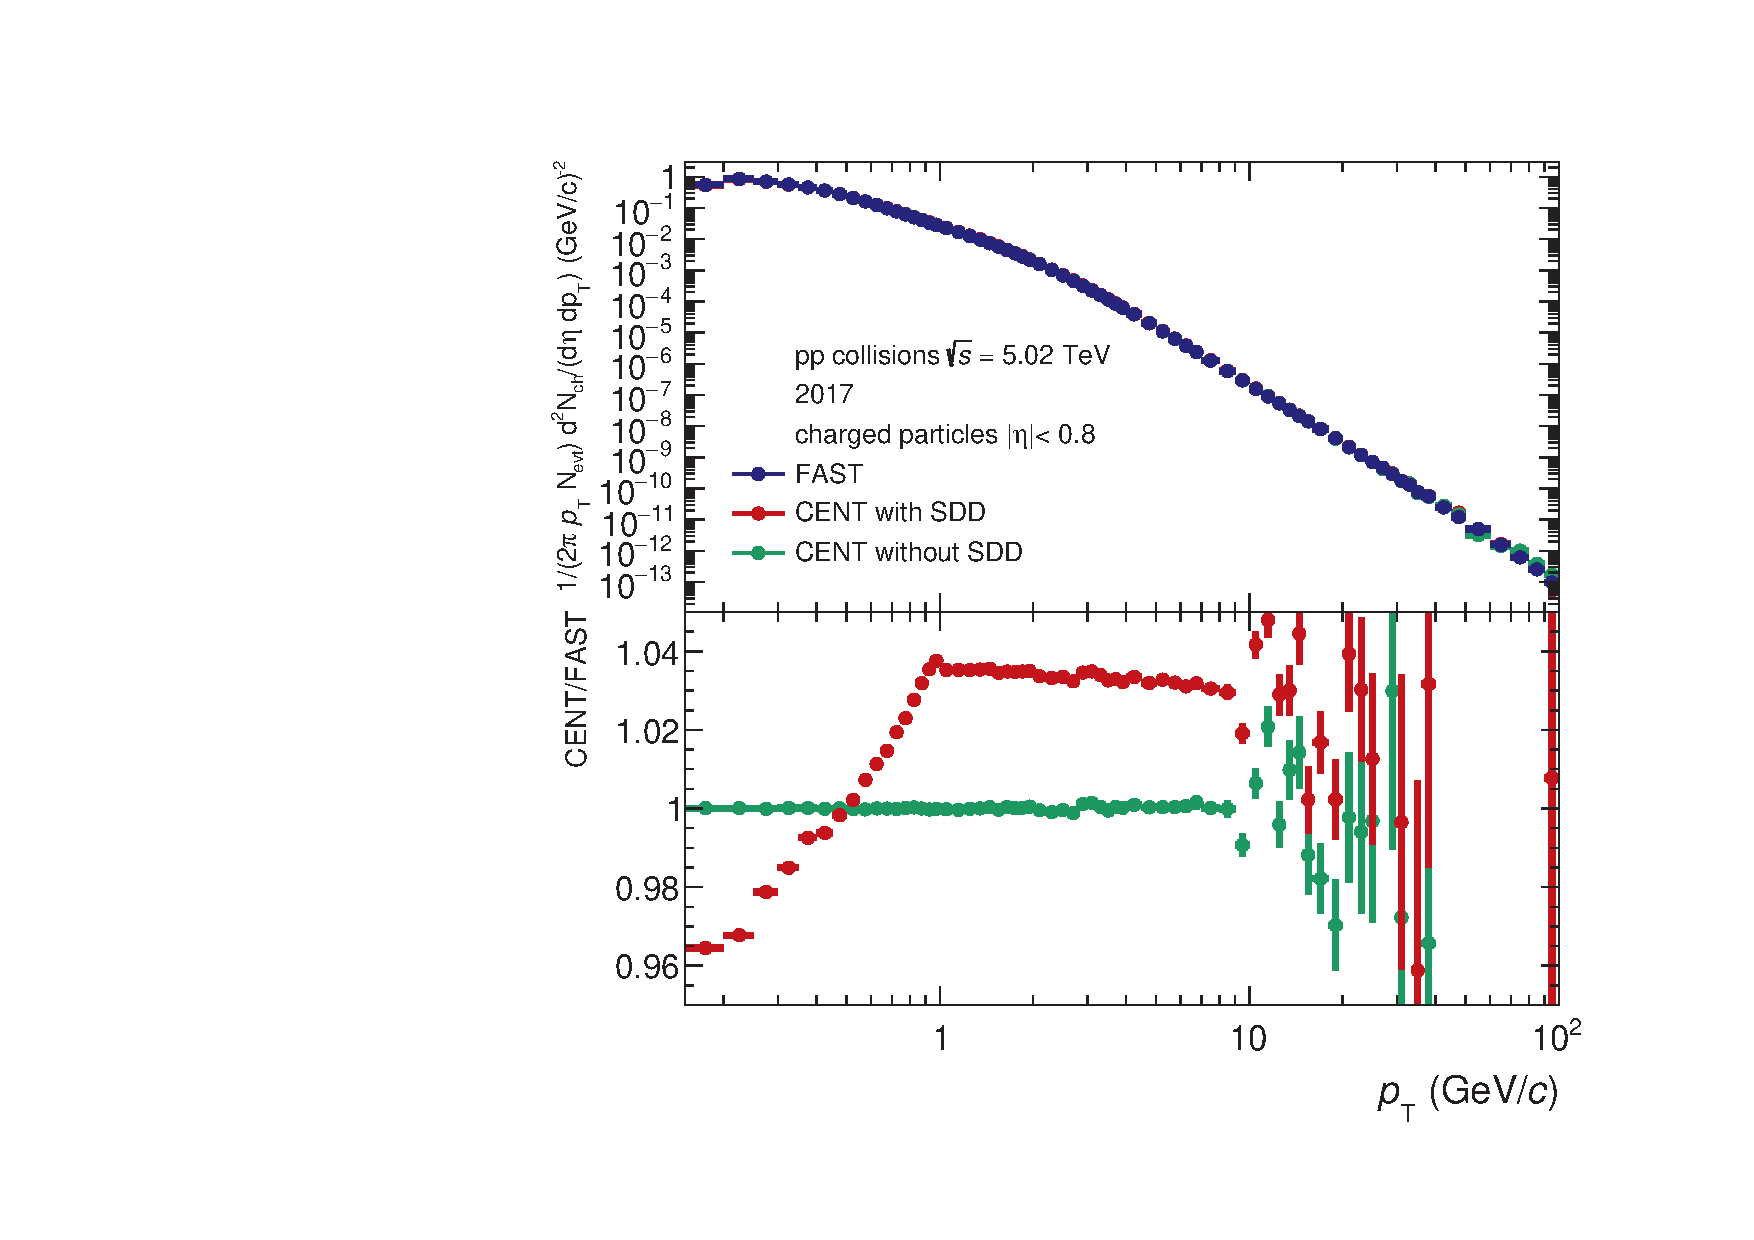
\includegraphics[width=11cm]{Plots/uncorrectedSpectra.pdf} 
\caption{Unkorrigierte $p_{\mathrm{T}}$-Spektren aus den Datensätzen \textsc{FAST} und \textit{CENT} mit und ohne SDD.}
\label{RawSpectra}
\end{figure}
\vspace{-0.5cm}
\subsection{Nachweiseffizienz geladener Teilchen}
Das benutzte Detektorsystem kann aufgrund seiner Beschaffenheit sowie von der Akzeptanz geladene Spuren mit einer bestimmten Wahrscheinlichkeit nachweisen. So kommt es zum Beispiel gelegentlich vor, dass der Rekonstruktionsalgorithmus, der aus den mit den Detektoren gemessenen Signalen eine Spur rekonstruieren soll, nicht in der Lage ist, eine Spur zu finden, oder aber eine Spur rekonstruiert, die den Selektionskriterien nicht entspricht und daher verworfen wird. Dies impliziert die Existenz einer gewissen Nachweiseffizienz des Detektors $\epsilon_{\mathrm{N}}$, die entsprechend korrigiert werden kann. Solche eine Korrektur betrifft per Definition die Spuren \cite{Acharya:2018qsh}.\\
Die Nachweiseffizienz hängt von den vier kinematischen Variablen einer geladenen Spur ab: dem Transversalimpuls $p_{\mathrm{T}}$, der Pseudorapidität $\eta$, dem Kollisionsvertex $V_{Z}$ und der Multiplizität $N_{ch}$. Außerdem ist anzumerken, dass die Nachweiseffizienz eine Abhängigkeit von der Teilchensorte zeigt. Die von den Monte-Carlo-Simulationen gelieferten Informationen werden dann verwendet, um das Verhältnis von rekonstruierten Spuren zu generierten Primärteilchen zu berechnen, aus dem sich die Nachweiseffizienz $\epsilon_{\mathrm{N}}$ ergibt:
\begin{equation} \label{eq:TrackingEff}
  \epsilon_{\mathrm{N}}=\dfrac{N^{MC}_{prim,rek}(p_{\mathrm{T}}, \eta, V_{Z}, N_{ch})}{N^{MC}_{prim,gen}(p_{\mathrm{T}}, \eta, V_{Z}, N_{ch})}
\end{equation}
\begin{figure}[tb!]
\centering
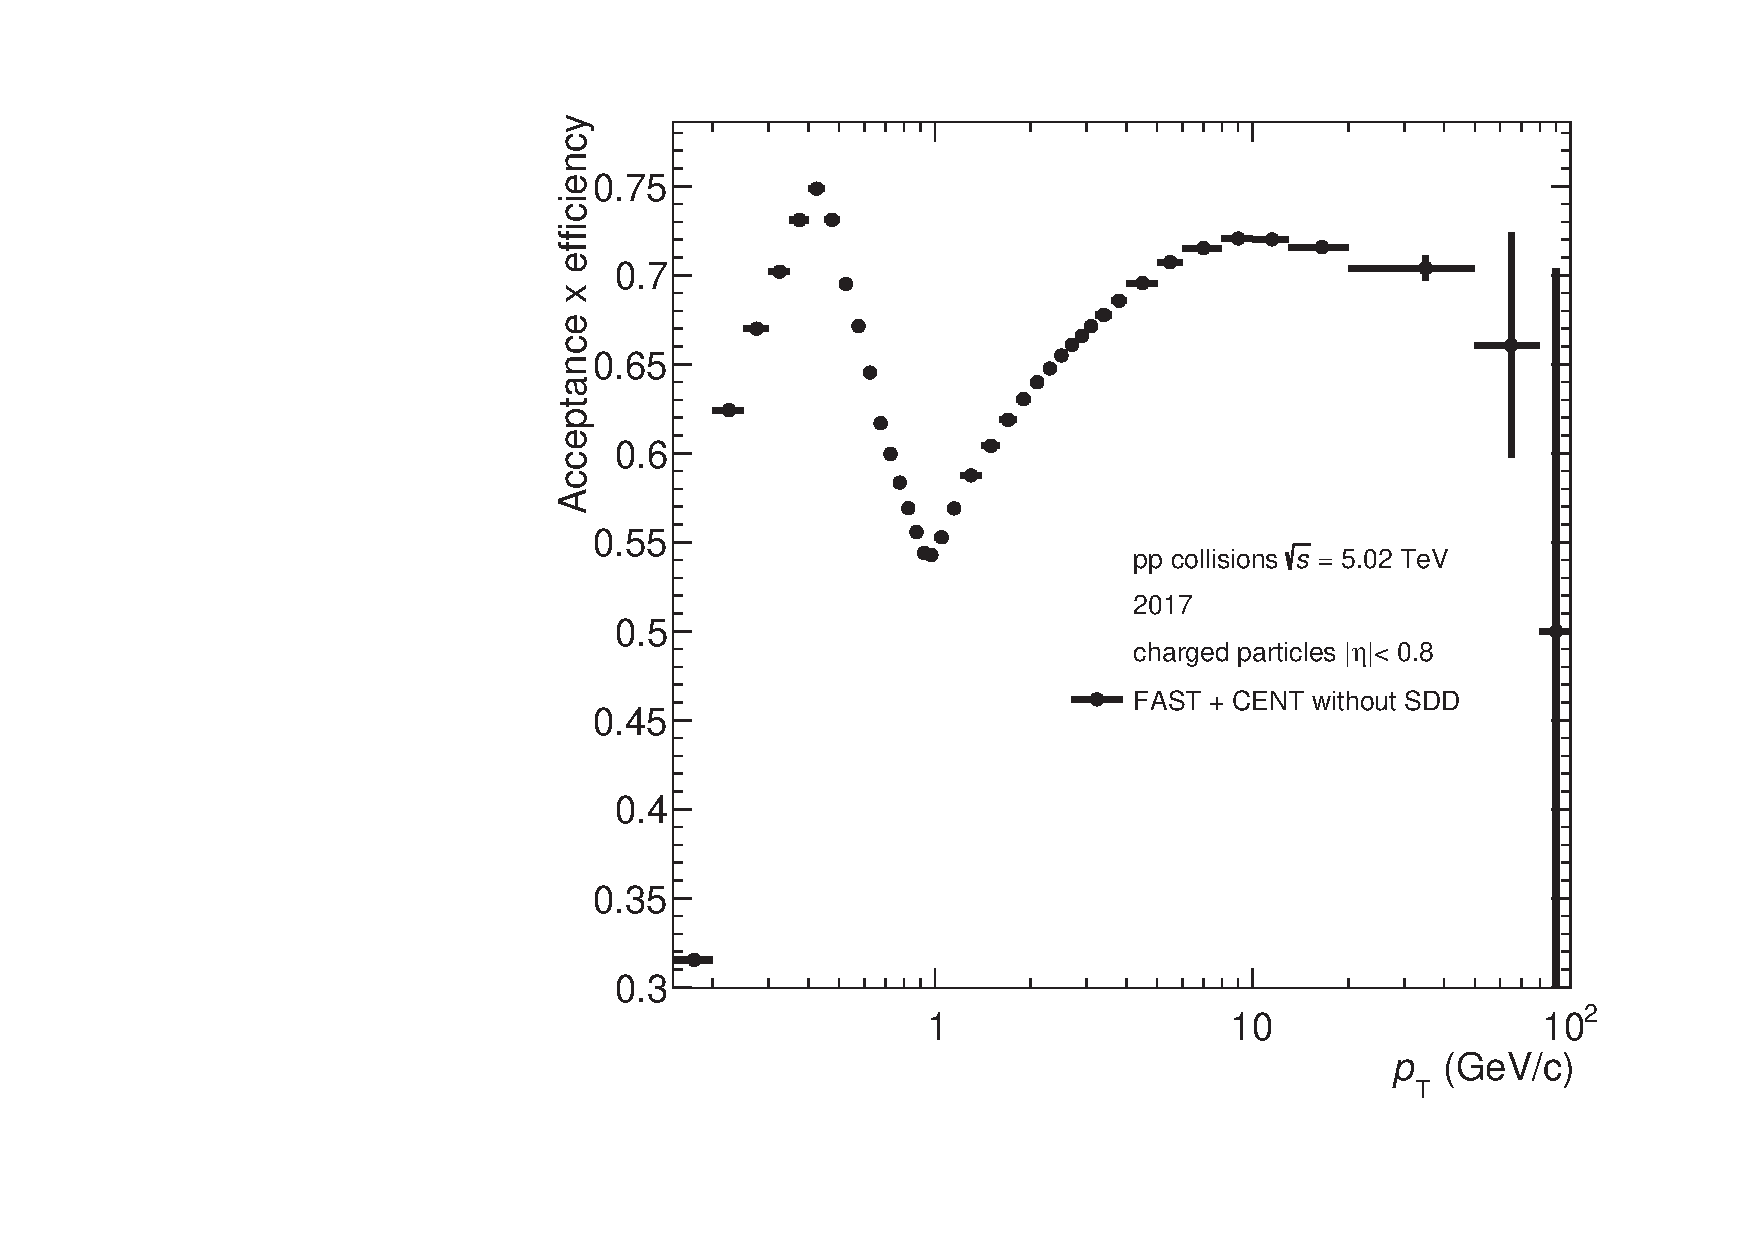
\includegraphics[width=11cm]{Plots/trackingEfficiency.pdf}  
\caption{Nachweiseffizienz in Abhängigkeit des Transversalimpulses $p_{\mathrm{T}}$ geladener Teilchen in simulierten pp-Kollisionen mithilfe von PYTHIA und GEANT3.}
\label{TrackingEff}
\end{figure}
\hspace{-0.1cm}In der Abbildung \ref{TrackingEff} ist die aus der Kombination der Datensätze \textsc{FAST} und \textit{CENT} ohne SDD erhaltene Nachweiseffizienz als Funktion des Transversalimpulses $p_{\mathrm{T}}$ abgebildet. Insgesamt beobachtet man, dass die Nachweiseffizienz in einem Bereich zwischen $50$ \% und $75$ \% liegt. Es fällt auch auf, dass die Kurve bei niedrigem $p_{\mathrm{T}}$, d.h. zwischen $0.15$ $\mathrm{GeV}/c$ und $0.3$ $\mathrm{GeV}/c$, eine steigende Tendenz hat. Erklären lässt sich dieses Wachstum mit der starken Krümmung, die Spuren in diesem konkreten $p_{\mathrm{T}}$-Intervall wegen des magnetischen Feldes sowie des Energieverlustes beim Durchlauf durch das Material aufweisen. Dieses Phänomen erleichtert den Nachweis des Teilchens bei niedrigem $p_{\mathrm{T}}$ und bewirkt somit den Anstieg. Bei rund \hspace{4cm} $p_{\mathrm{T}} \thickapprox 1$ $\mathrm{GeV}/c$ beobachtet man allerdings eine bemerkenswerte Abnahme der Nachweiseffizienz, welche durch das Kriterium verursacht wird, dass die Spuren eine minimale geometrische Länge in einem TPC Teilbereich besitzen müssen (siehe Tabelle \ref{tab:Cuts}). Da die sich in diesem $p_{\mathrm{T}}$-Bereich befindenden Primärteilchen dazu neigen, die TPC durch die Ränder zu durchqueren, werden die jeweiligen Spuren durch das erwähnte Kriterium ausgeschlossen. Dies führt zu einer weniger effektiven Rekonstruktion der Spuren. Letztendlich erreicht die Nachweiseffizienz mit steigendem $p_{\mathrm{T}}$ und nach einer progressiven Zunahme ein Plateau von rund $70\%$ bei $p_{\mathrm{T}} > 10$ $\mathrm{GeV}/c$.
\subsection{Abschätzung der Kontamination durch Sekundärteilchen}
\begin{figure}[H]
\centering
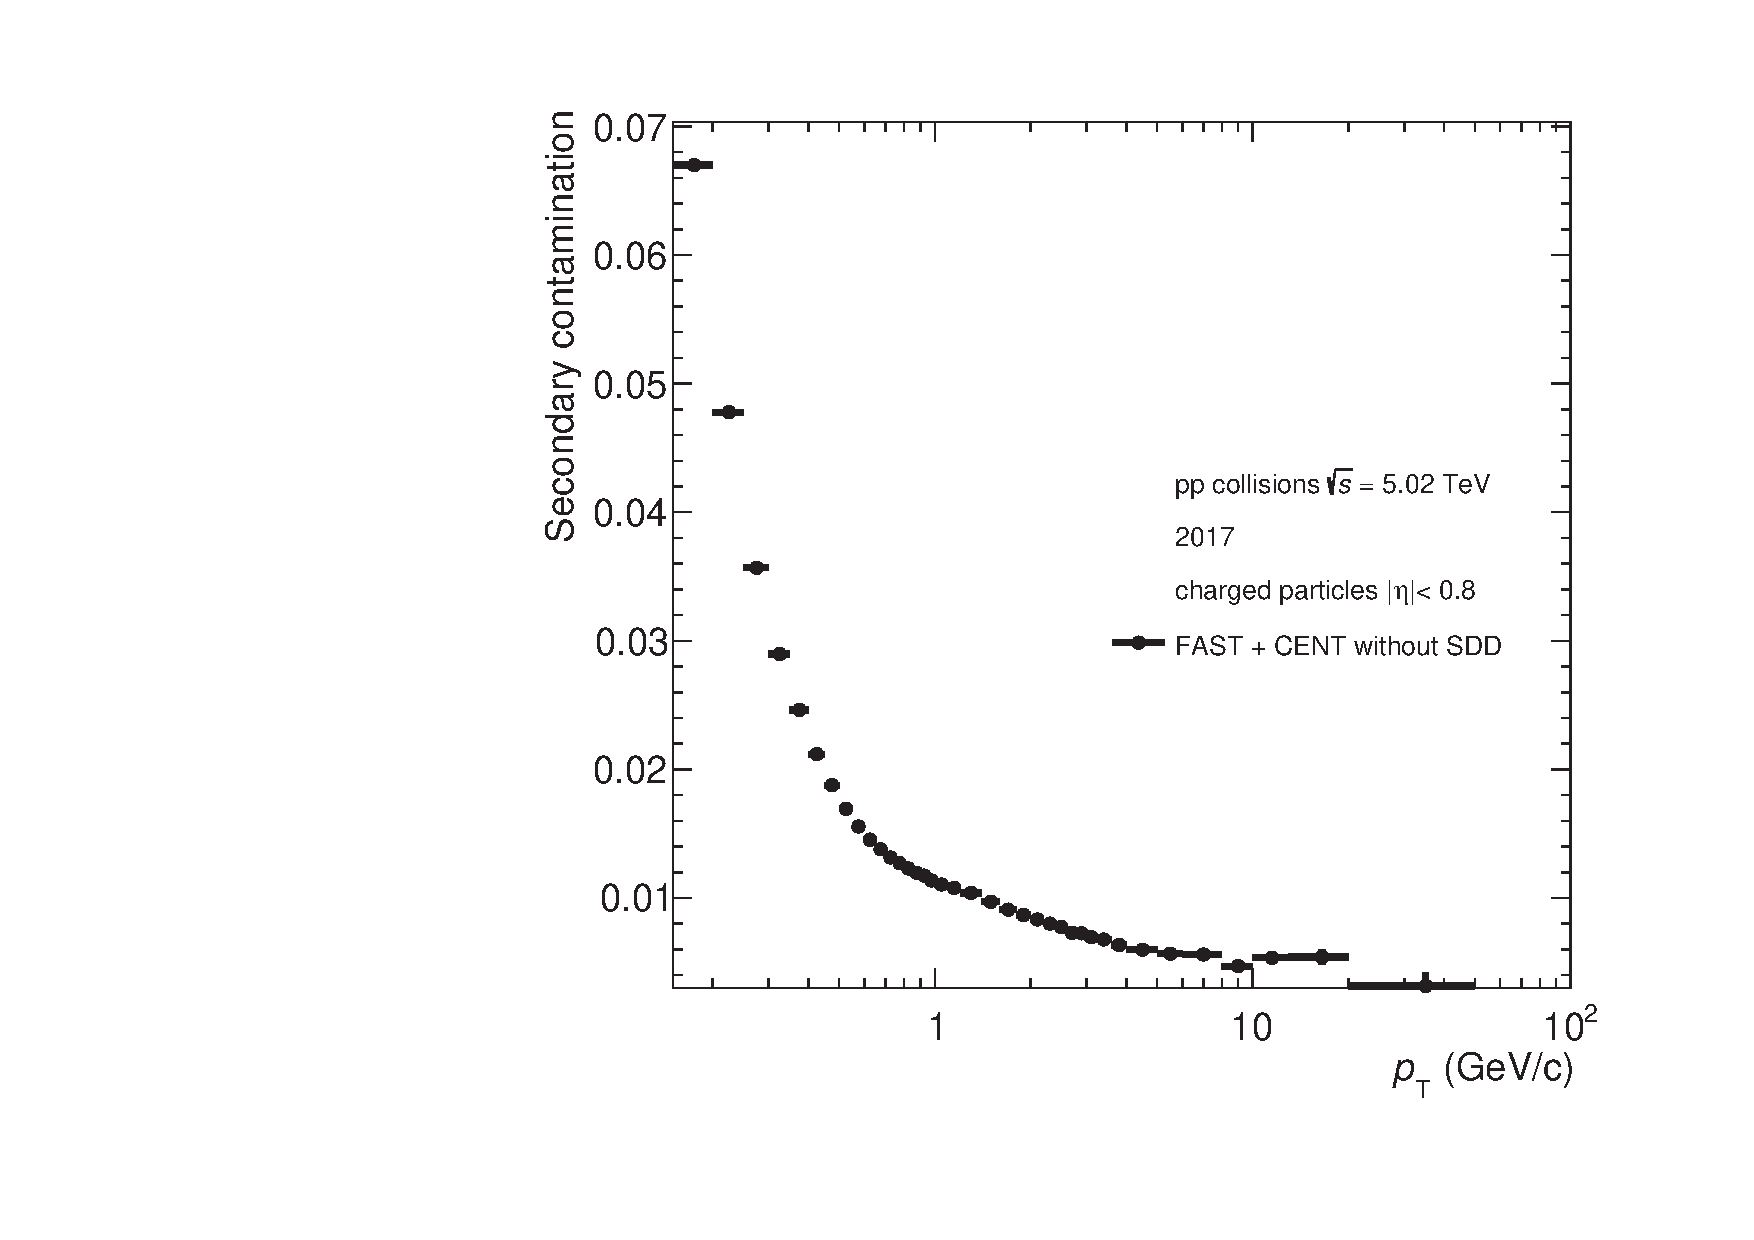
\includegraphics[width=11cm]{Plots/SecCont.pdf}  
\caption{Anteil der sekundären geladenen Teilchen in Abhängigkeit des Transversalimpulses $p_{\mathrm{T}}$.}
\label{SecCont}
\end{figure}
Die im Unterkapitel \ref{sec:Spurselektion} beschriebenen Spurselektionen zielen unter anderem darauf ab, die Kontamination der gemessenen Daten durch Sekundärteilchen zu minimieren. Trotzdem bleibt ein kleiner Anteil übrig. Dies fordert die Anwendung einer Korrektur, die den genannten Anteil aus den Daten extrahiert.\\
Wie schon angesprochen, werden den Sekundärteilchen Teilchen zugeordnet, die nicht unmittelbar mit der Kollision zusammenhängen, sondern die aus schwachen Zerfällen stammen, wie. z.B. aus Zerfälle von neutralen Kaonen $K^{0}$, von Lambda-Baryonen $\Lambda$ oder seltener von Myonen $\mu$. Neben solchen Fällen sind auch Teilchen, die aus Wechselwirkungen mit dem Detektormaterial resultieren, als sekundär definiert.\\
Zur Bestimmung des Anteils von Sekundärteilchen, der im gemessenen $p_{\mathrm{T}}$-Spektrum vorhanden ist, bedient man sich den Monte-Carlo-Simulationen. In der Abbildung \ref{SecCont} wird die Verteilung 
von diesem Anteil als Funktion des Transversalimpulses $p_{\mathrm{T}}$ dargestellt. Man beobachtet, dass die Anzahl sekundärer Teilchen $7$ \% der Gesamtzahl von Teilchen nicht übersteigt. Die Kurve zeigt ein tendenziell fallendes Verhalten, welches darauf zurückzuführen ist, dass Zerfallsprodukte oder Teilchen, die mit dem Detektormaterial wechselwirken, kleinere Transversalimpulse aufgrund der Energieverluste während der verschiedenen Prozesse aufweisen.
\subsection{$p_{\mathrm{T}}$-Auflösung}
Der Transversalimpuls geladener Teilchen wird aus der durch das Magnetfeld bedingten Krümmung ihrer Spur berechnet. Hierbei verhält sich die Krümmung proportional zum Kehrwert des Transversalimpulses $1/p_{\mathrm{T}}$. Teilchen mit hohen Transversalimpulsen haben geradere Spuren, welche mit den ALICE-Detektoren schwierig rekonstruiert werden können. Dies schlägt sich in einer Messunsicherheit $\sigma(1/p_{\mathrm{T}})$ nieder. Die Auswirkung dieser Unsicherheit wird stärker bei hohen Transversalimpulsen. Zudem lassen sich Spuren positiv und negativ geladener Teilchen unterschiedlich rekonstruieren, was auch zur genannten Messunsicherheit beiträgt. Aus diesem Grund ist das gemessene $p_{\mathrm{T}}$-Spektrum verschmiert und eine entsprechende Korrektur wird daher notwendig.\\
Die relative $p_{\mathrm{T}}$-Auflösung $\sigma(p_{\mathrm{T}})/p_{\mathrm{T}}$ in Abhängigkeit des Transversalimpulses lässt sich wie folgt bestimmen \cite{knichel2015transverse}:
\begin{equation} \label{eq:RelativePtResolution}
  \dfrac{\sigma(p_{\mathrm{T}})}{p_{\mathrm{T}}} \approx p_{\mathrm{T}} \cdot \sigma(1/p_{\mathrm{T}})
\end{equation}
Dabei bezeichnet $\sigma(1/p_{\mathrm{T}})$ die Unsicherheit, den Kehrwert des Transversalimpulses $1/p_{\mathrm{T}}$ zu messen, wie schon angesprochen. Abbildung \ref{RelativePtResolution} stellt die mittlere relative $p_{\mathrm{T}}$-Auflösung als Funktion von $p_{\mathrm{T}}$ für die in dieser Arbeit verschiedenen verwendeten Datensätze dar. Man beobachtet, dass die jeweiligen Verteilungen sehr ähnliche Verläufe besitzen. Bei $p_{\mathrm{T}} \thickapprox 1$ $\mathrm{GeV}/c$ befindet sich das Minimum der Verteilungen mit $\left<\sigma(p_{\mathrm{T}})/p_{\mathrm{T}}\right> \thickapprox 1$ \%. Dies ist die bestmögliche Auflösung im gesamten $p_{\mathrm{T}}$-Bereich. Bei hohen Transversalimpulsen verschlechtert sich die Auflösung und erreicht für $p_{\mathrm{T}}=50$ GeV/\textit{c} Werte von rund $4$ \%. Ab diesem Punkt werden die Fluktuationen aufgrund der geringer werdenden Statistik immer stärker. Anhand dieser Abbildung kann man zusätzlich bestätigen, dass die Ereignisse von \textit{FAST} und \textit{CENT} ohne SDD kombiniert werden dürfen, denn die jeweiligen Verteilungen haben wieder einen praktisch identischen Verlauf.\\
Des Weiteren fällt es auf, dass \textit{FAST} ab $p_{\mathrm{T}} \approx 1$ GeV/\textit{c} eine bessere $p_{\mathrm{T}}$-Auflösung als \textit{CENT} mit SDD aufweist. Dies widerspricht allerdings der intuitiven Annahme, dass eine bessere $p_{\mathrm{T}}$-Auflösung beim Einsatz der SDD-Schichten zu erwarten ist, da es in diesem Fall mehr Spurpunkte zur Rekonstruktion der Spur gibt. Das kann daran liegen, dass sich die Anfangsbedingungen der Messung der jeweiligen Datensätze unterscheiden. Eine ungleiche Kalibrierung des ITS könnte beispielsweise diese unerwartete Abweichung verursachen.\\
Aufgrund der $p_{\mathrm{T}}$-Auflösung entspricht das gemessene $p_{\mathrm{T}}$-Spektrum nicht der wahren $p_{\mathrm{T}}$-Verteilung. Das gemessene $p_{\mathrm{T}}$-Spektrum resultiert in der Tat aus einer Faltung des wahren $p_{\mathrm{T}}$-Spektrums mit einer Funktion $R(p_{\mathrm{T}})$, die zu einem gegebenen wahren Transversalimpuls die statistische Verteilung des gemessenen Transversalimpulses angibt:
\begin{equation} 
  \left(\dfrac{\mathrm{d}^2 N_{ch}}{\mathrm{d}p_{\mathrm{T}} \mathrm{d}\eta} \right)_{\mathrm{gemessen}} (p_{\mathrm{T}}) = \left(\left(\dfrac{\mathrm{d}^2 N_{ch}}{\mathrm{d}p_{\mathrm{T}} \mathrm{d}\eta} \right)_{\mathrm{wahr}} *R \right)(p_{\mathrm{T}})
\end{equation}
\begin{figure}
\centering
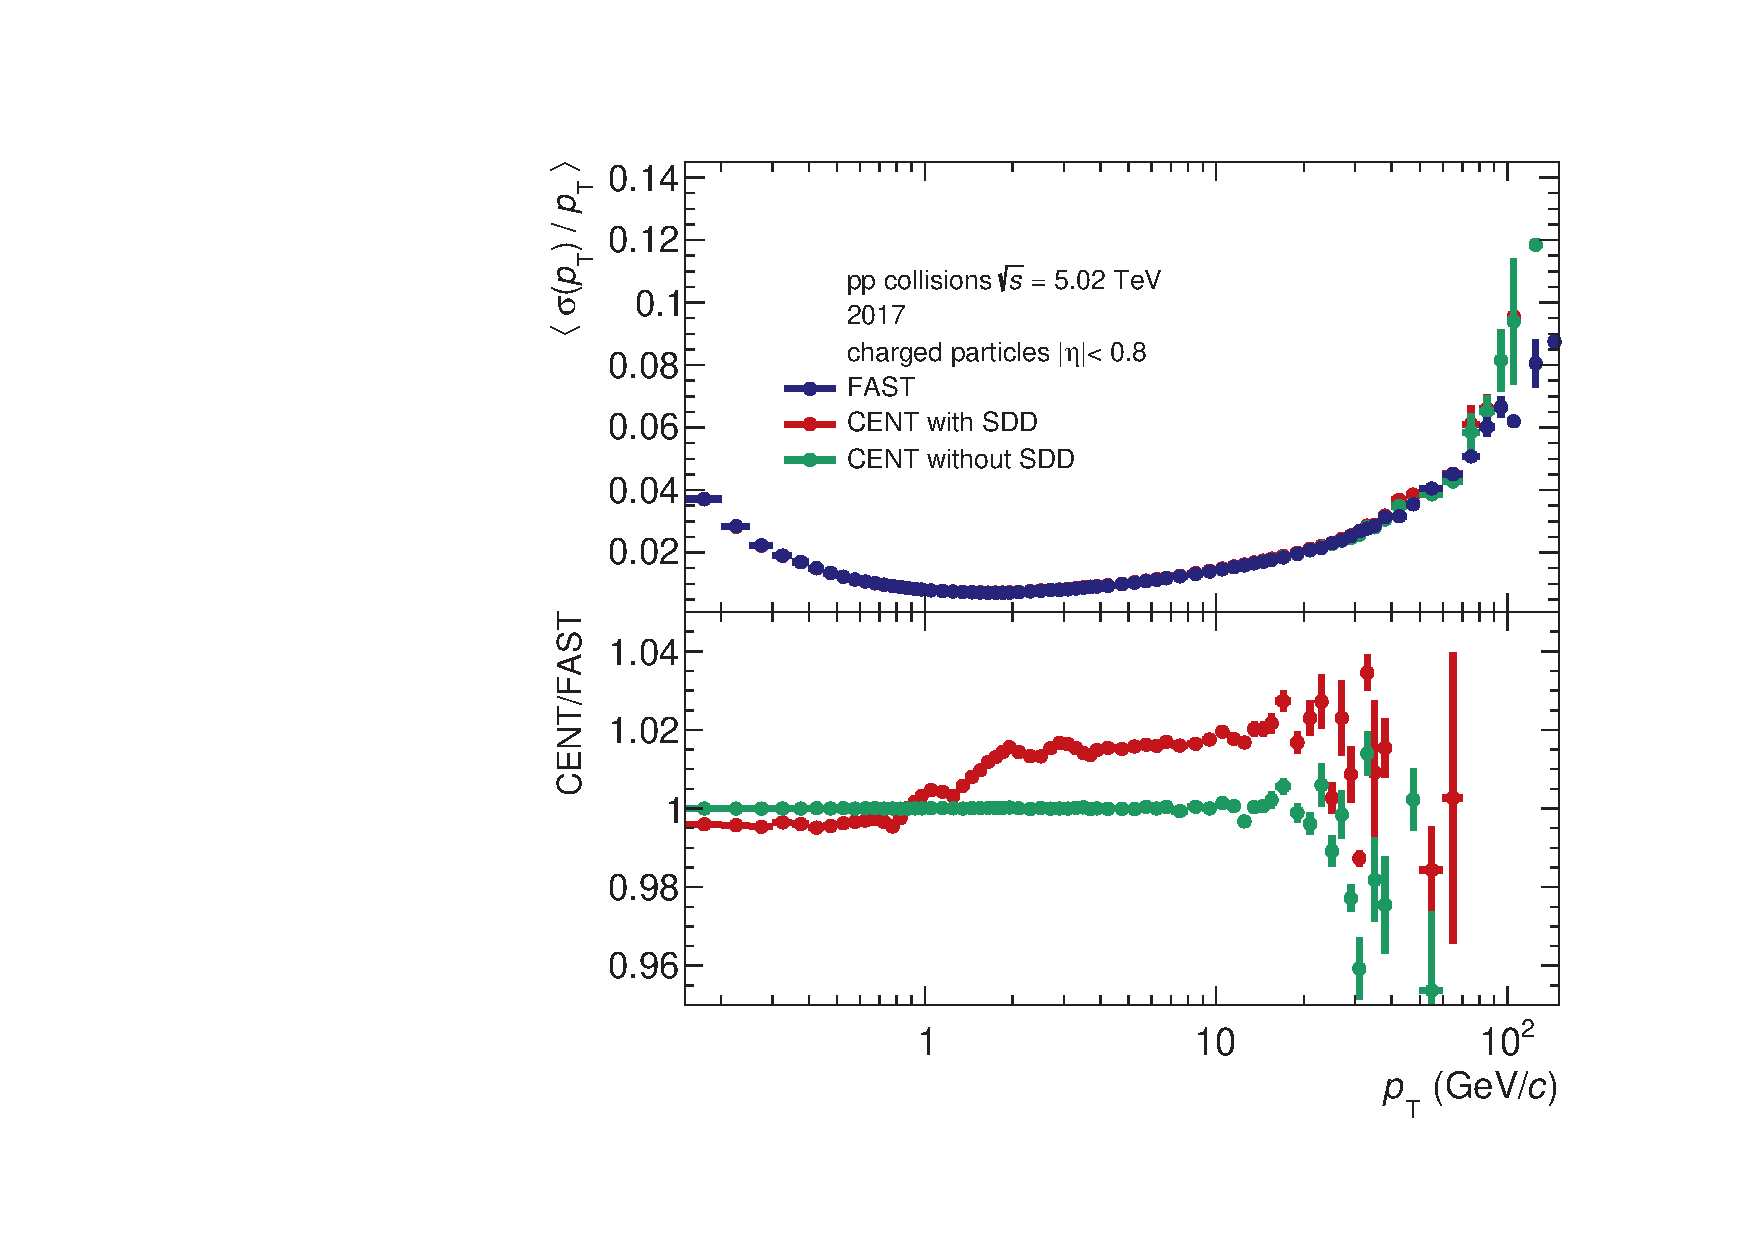
\includegraphics[width=11cm]{Plots/pTResolution.pdf}  
\caption{Mittlere relative $p_{\mathrm{T}}$-Auflösung als Funktion des Transversalimpulses.}
\label{RelativePtResolution}
\end{figure}
\hspace{-0.25cm} Die $R(p_{\mathrm{T}})$-Funktion fasst alle Detektoreffekte auf die $p_{\mathrm{T}}$-Auflösung zusammen. Zur Bestimmung des wahren $p_{\mathrm{T}}$-Spektrums wird ein $p_{\mathrm{T}}$-abhängiger Korrekturfaktor auf das gemessene $p_{\mathrm{T}}$-Spektrum angewendet. Dieser Korrekturfaktor beschreibt den Zusammenhang zwischen beiden $p_{\mathrm{T}}$-Spektren und ist als das Verhältnis vom wahren zum gemessenen $p_{\mathrm{T}}$-Spektrum definiert. Da sich der Korrekturfaktor auf das gemessene $p_{\mathrm{T}}$-Spektrum kaum auswirkt, kann angenommen werden, dass dieser Korrekturfaktor ähnlich zum Verhältnis vom gemessenen zum mit $R(p_{\mathrm{T}})$ gefalteten gemessenen $p_{\mathrm{T}}$-Spektrum ist:
\begin{equation} 
  \footnotesize C_{\mathrm{Aufloesung}}(p_{\mathrm{T}}) = \dfrac{\left(\dfrac{\mathrm{d}^2 N_{ch}}{\mathrm{d}p_{\mathrm{T}} \mathrm{d}\eta} \right)_{\mathrm{wahr}}}{\left(\dfrac{\mathrm{d}^2 N_{ch}}{\mathrm{d}p_{\mathrm{T}} \mathrm{d}\eta} \right)_{\mathrm{gemessen}}}(p_{\mathrm{T}})  \approx \dfrac{ \left(\dfrac{\mathrm{d}^2 N_{ch}}{\mathrm{d}p_{\mathrm{T}} \mathrm{d}\eta} \right)_{\mathrm{gemessen}} }{\left(\left(\dfrac{\mathrm{d}^2 N_{ch}}{\mathrm{d}p_{\mathrm{T}} \mathrm{d}\eta} \right)_{\mathrm{gemessen}} *R \right)}(p_{\mathrm{T}}) 
\end{equation}

\begin{figure}[tb!]
\centering
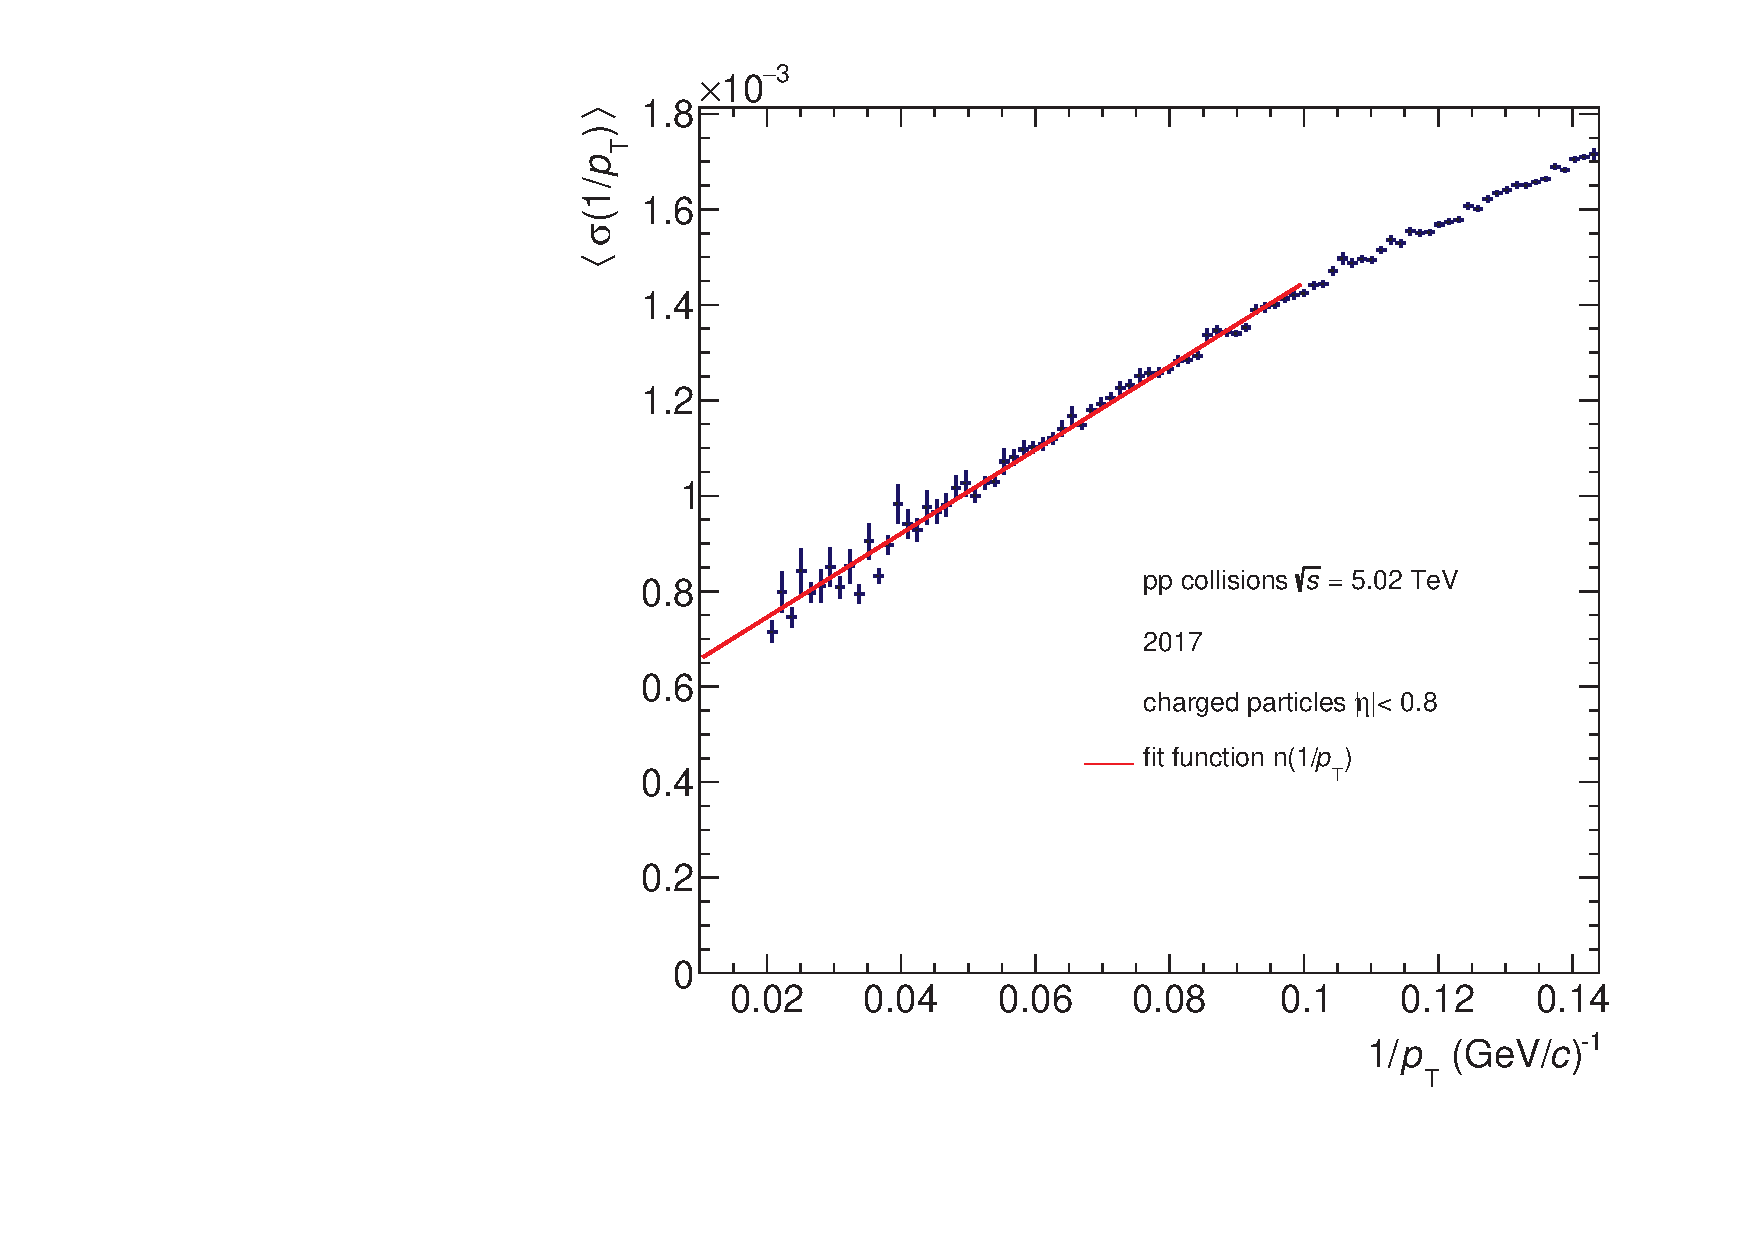
\includegraphics[width=0.495\textwidth]{Plots/fitfunc.pdf}  
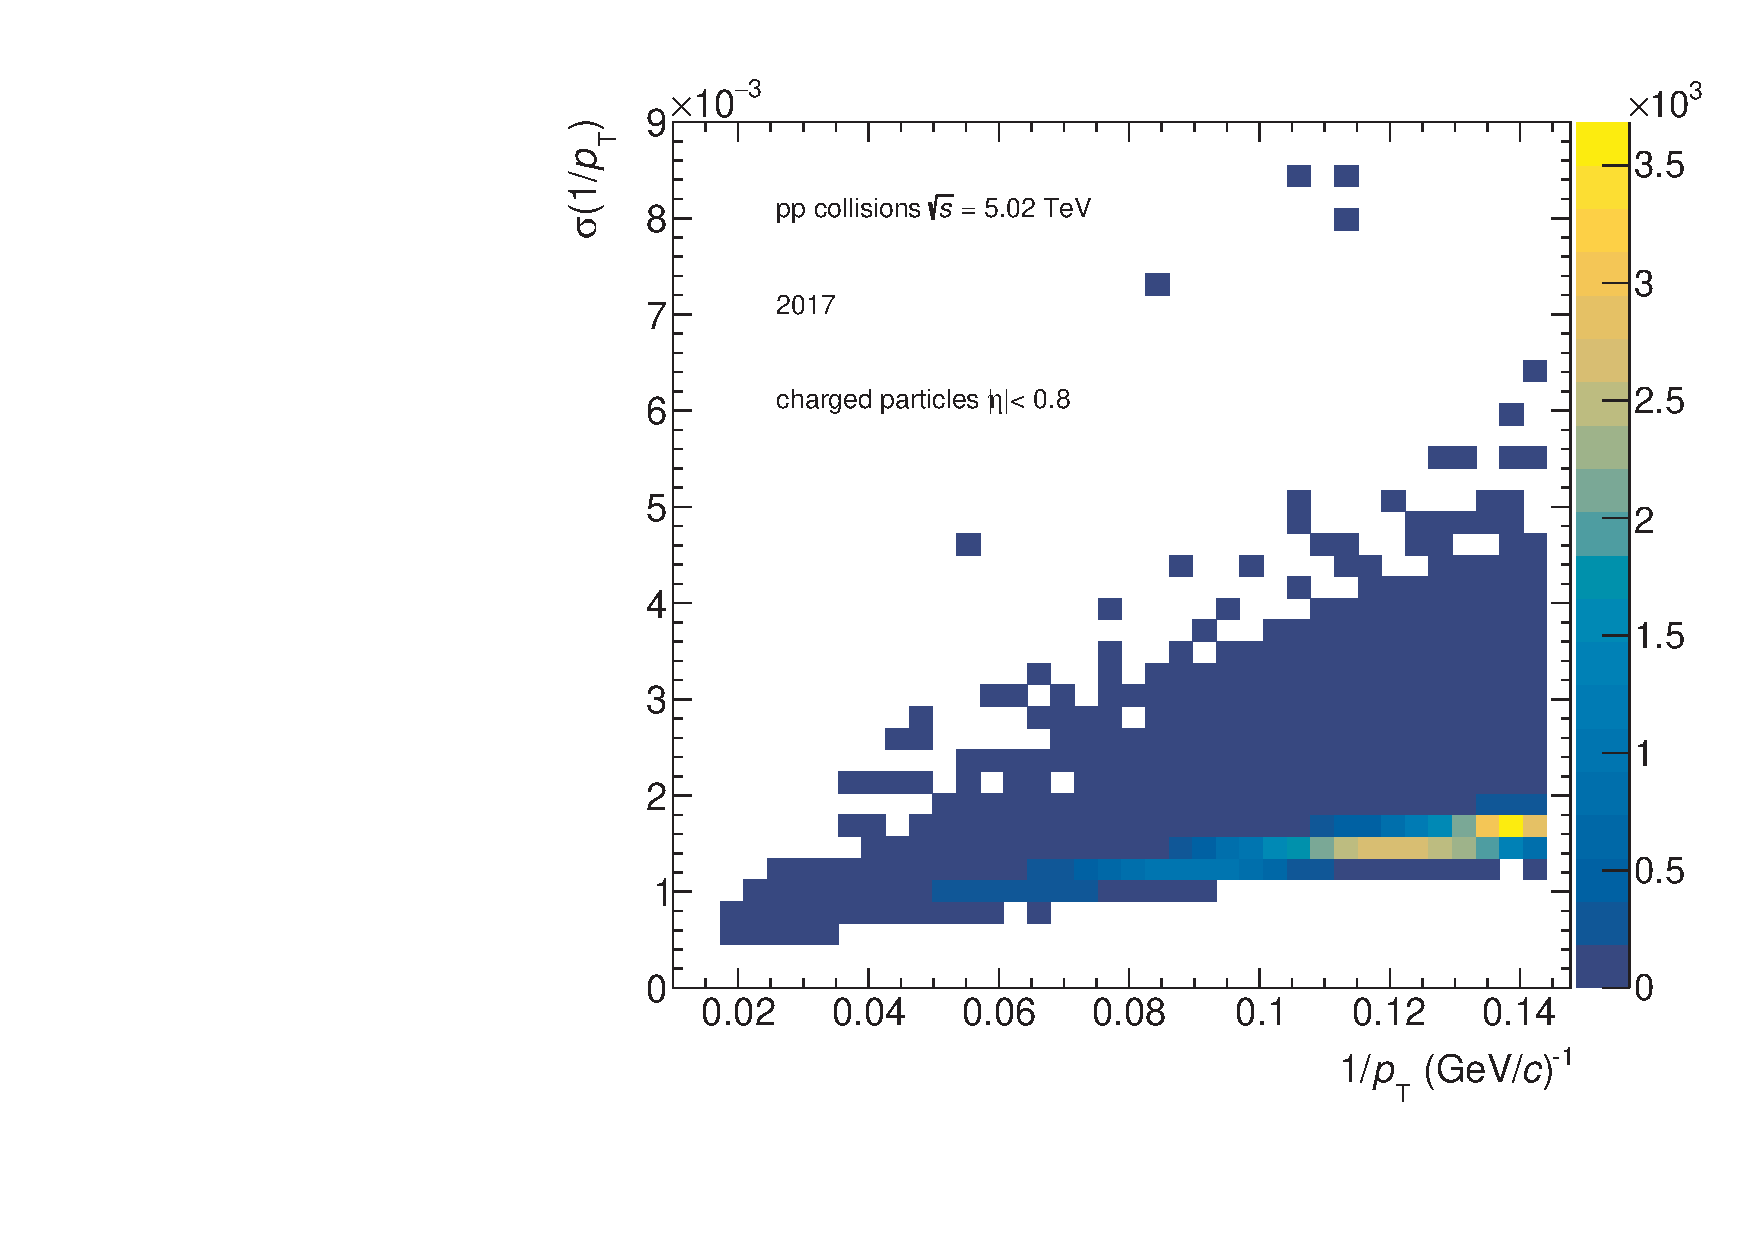
\includegraphics[width=0.495\textwidth]{Plots/reso2dim.pdf}  
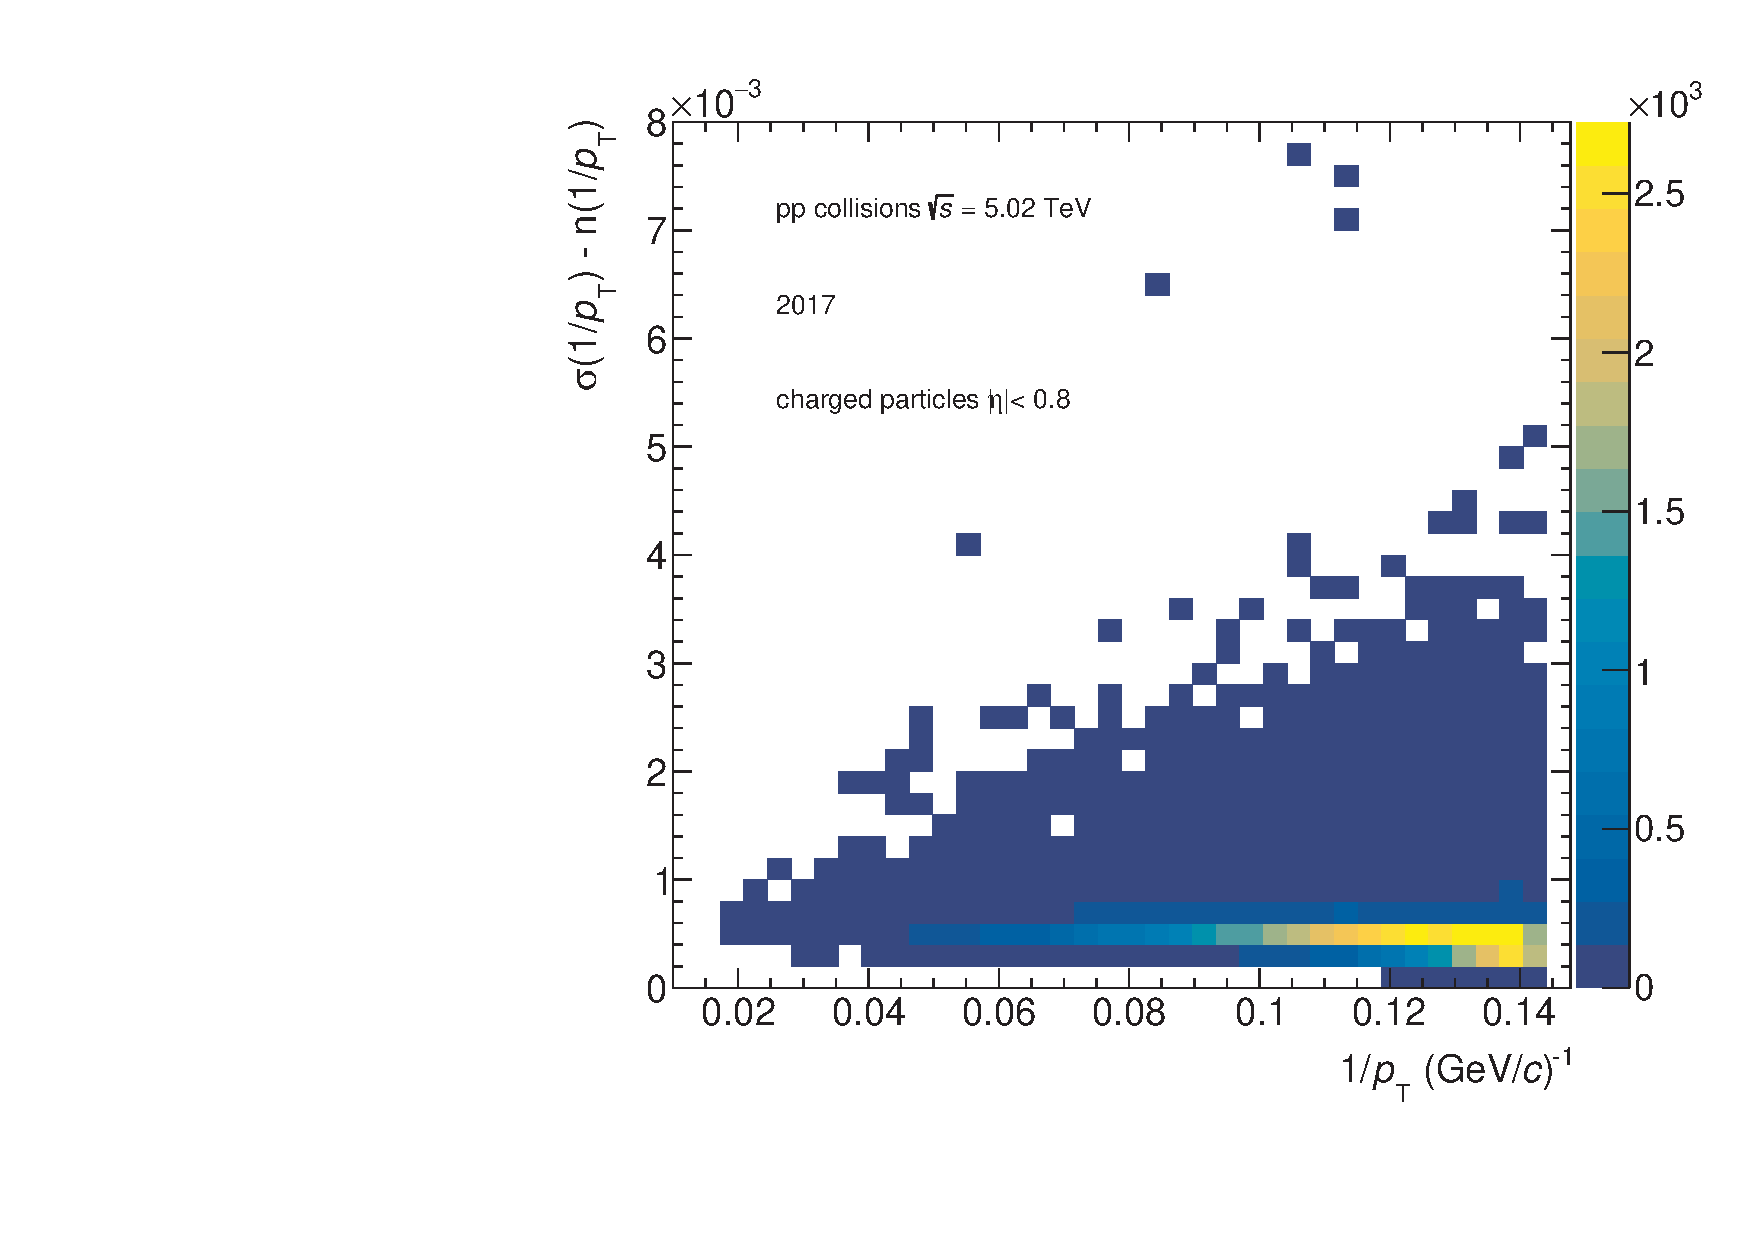
\includegraphics[width=0.495\textwidth]{Plots/scaledcov.pdf}  
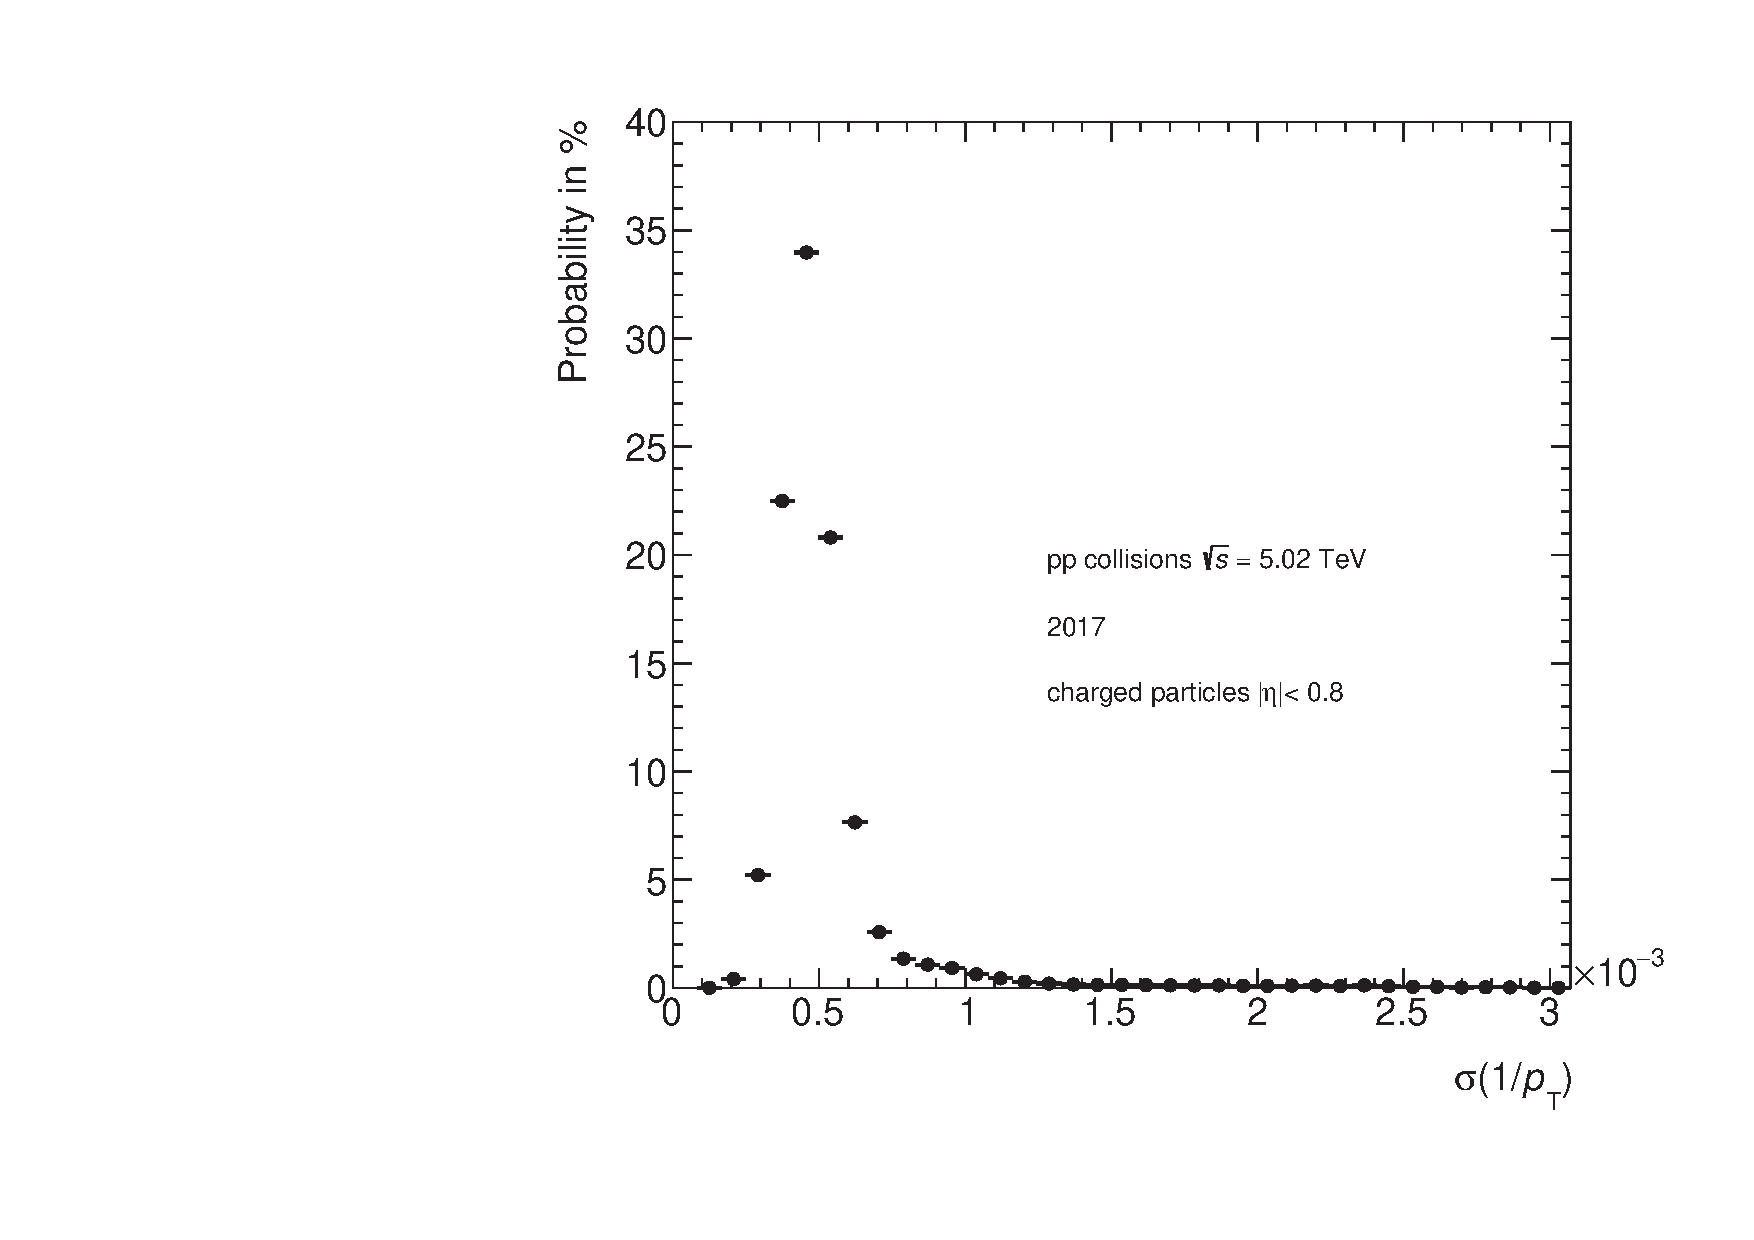
\includegraphics[width=0.495\textwidth]{Plots/confunction.pdf}  
\caption{\textbf{Oben.} Links: $p_{\mathrm{T}}$-Auflösung als Funktion von $1/p_{\mathrm{T}}$. Rechts: Parametrisierung $n(1/p_{\mathrm{T}})$ der mittleren $p_{\mathrm{T}}$-Auflösung als Funktion von $1/p_{\mathrm{T}}$. \textbf{Unten.} Links: Skalierte $p_{\mathrm{T}}$-Auflösung als Funktion von $1/p_{\mathrm{T}}$. Rechts: Darstellung der flächennormierten statistischen Verteilung der $p_{\mathrm{T}}$-Auflösung als Funktion von $1/p_{\mathrm{T}}$.}
\label{4plots}
\end{figure}

\begin{figure}[tb!]
\centering
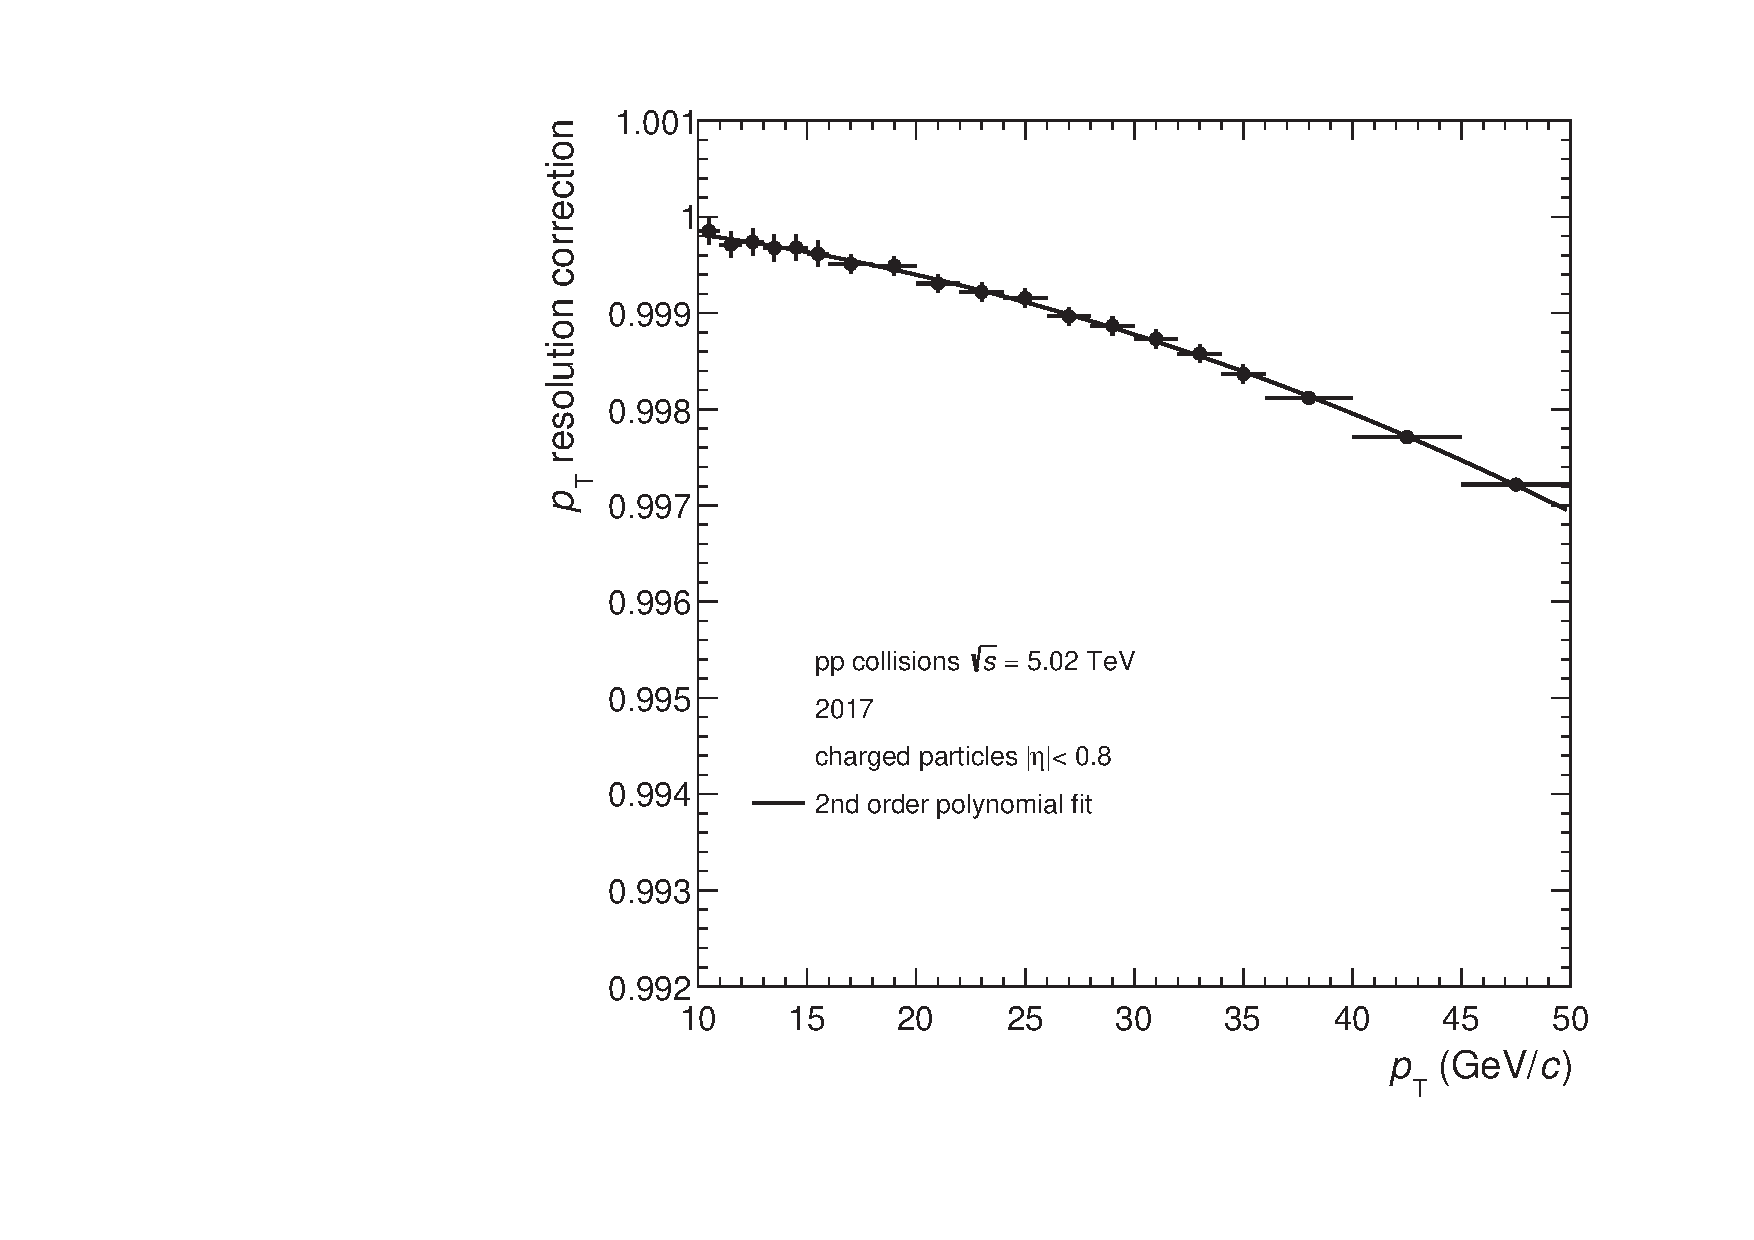
\includegraphics[width=9cm]{Plots/corrResFactor.pdf}  
\caption{Parametrisierter Korrekturfaktor der $p_{\mathrm{T}}$-Auflösung als Funktion des Transversalimpulses.}
\label{corrResFactor}
\end{figure}

Zur Berechnung des Korrekturfaktors der $p_{\mathrm{T}}$-Auflösung soll dementsprechend das gemessene $p_{\mathrm{T}}$-Spektrum mit der $R(p_{\mathrm{T}})$-Funktion gefaltet werden. Da sie nicht bestimmt werden kann, wird eine Simulation benutzt, deren Verfahren im Folgenden detailliert beschrieben wird. Die Simulation ist in der Lage, die Auswirkung der $R(p_{\mathrm{T}})$-Funktion zu reproduzieren.\\
Zu diesem Zweck wird zuerst die mittlere $p_{\mathrm{T}}$-Auflösung als Funktion von $1/p_{\mathrm{T}}$ mit einer Polynomfunktion zweiter Ordnung parametrisiert (siehe Abbildung \ref{4plots} oben links). Anschließend wird die von $1/p_{\mathrm{T}}$ abhängigen $p_{\mathrm{T}}$-Auflösung im Intervall $7 < p_{\mathrm{T}} < 50$ GeV/\textit{c} berücksichtigt (siehe Abbildung \ref{4plots} oben rechts). Die obengenannte Parametrisierung wird dann aus dieser Verteilung abgezogen. Dadurch werden statistische Fluktuationen bei großen Transversalimpulsen vermieden. Die sich daraus ergebende skalierte $p_{\mathrm{T}}$-Auflösung (siehe Abbildung \ref{4plots} unten links) wird danach auf die Ordinatenachse projiziert. Als Ergebnis erhält man die benötigte statistische Verteilung von $\sigma(1/p_{\mathrm{T}})$ (siehe Abbildung \ref{4plots} unten rechts). An dieser Stelle soll darauf hingewiesen werden, dass die letzte Abbildung lediglich die Form dieser Verteilung zeigt. Die exakte Position der jeweiligen Anhäufung hängt von $1/p_{\mathrm{T}}$ ab und wird daher an jedem Punkt entsprechend der oben erwähnten Parametrisierung bestimmt.\\ 
Die Faltung wird zuerst auf ein $1/p_{\mathrm{T}}$-Spektrum angewendet, indem man jeder einzelner Datenpunkt gemäß einer Gauß-Verteilung verschmiert, deren Standardabweichung mithilfe der statistischen Verteilung von $\sigma(1/p_{\mathrm{T}})$ zufällig erzeugt wird. Das Resultat lässt sich dann in das gefaltete gemessene $p_{\mathrm{T}}$-Spektrum umrechnen, das zur Bestimmung des Korrekturfaktors benutzt wird. Abbildung \ref{corrResFactor} zeigt den resultierenden Korrekturfaktor als Funktion von $p_{\mathrm{T}}$ im Intervall $10 < p_{\mathrm{T}} < 50$ GeV/\textit{c}. Der Korrekturfaktor besitzt ein monoton fallendes Verhalten und sein Minimalwert entspricht einer Abweichung des gemessenen zum wahren $p_{\mathrm{T}}$-Spektrum von $0.3$ \%.
\subsection{Normierung auf die Anzahl unelastischer Kollisionen}
Der in der vorliegenden Arbeit verwendete \textit{minimum bias} Trigger wirkt mit einer gewissen Effizienz. Trotz der hohen Effektivität des Triggers, kann die Art einer Kollision  nur mit einer Wahrscheinlichkeit beurteilt. Zum Beispiel kann er eventuell ein Ereignis als einen nicht-einfach diffraktiven Prozess aufzeichnen, wenn es in der Tat um einen einfach diffraktiven Prozess oder sogar um einen elastischen Stoß handelt. Für diesen Zweck muss das präsentierte $p_{\mathrm{T}}$-Spektrum auf die Anzahl von unelastischen Kollisionen $N_{unel}$ normiert werden. Dadurch werden physikalisch nicht relevante Kollisionen von der Analyse ausgeschlossen. Die resultierende Korrektur beeinflusst also im Unterschied zu den anderen Korrekturen nur die Anzahl der Ereignisse und hat somit keinen Effekt auf die Form der $p_{\mathrm{T}}$-Verteilung. Zur Anwendung dieser Korrektur wird folgenden Ausdruck verwendet:
\begin{equation}
\label{eq:Nunel}
	N_{\mathrm{unel}} = \dfrac{N_{V_{Z}<10}}{a_{V_{Z}<10} \cdot \epsilon_\mathrm{V} \cdot \epsilon_{\mathrm{MB}}}
\end{equation}
Dabei bezeichnet $N_{V_{Z}<10}$ die Anzahl von Ereignissen, deren Kollisionsvertices sich in einem Abstand kleiner als $10$ cm vom Nominalvertex $V_{Z} = 0$ entlang der Kollisionsachse befinden. Andererseits stellt $a_{V_{Z}<10}$ die Vertexakzeptanz, $\epsilon_\mathrm{V}$ die Vertexeffizienz und $\epsilon_{\mathrm{MB}}$ die \textit{minimum bias} Triggereffizienz.\\
Die Vertexakzeptanz stellt den Anteil von Ereignissen, die die festgestellte Selektion $|V_{Z}| < 10$ cm erfüllen, an der Anzahl rekonstruierter Ereignisse $N_{\mathrm{Rekon}}$ dar:
\begin{equation}
a_{V_{Z}<10} = \dfrac{N_{V_{Z}<10}}{N_{\mathrm{Rekon}}}
\end{equation}
Dieser Wert kann zwar mithilfe der Monte-Carlo-Simulationen berechnet werden, aber er lässt sich auch direkt aus der Messung bestimmen. Die zweite Variante liefert einen präziseren Wert als die erste und wird daher bevorzugt benutzt.\\
Die Vertexeffizienz ist durch das Verhältnis von Ereignissen mit Vertex $N_{Vtx}$ zu den Ereignissen $N_{\mathrm{MB}}$ definiert, die das \textit{minimum bias} Kriterium auslösten. Sie kann mithilfe der von den gemessenen Daten gelieferten Informationen wie folgt bestimmt werden:
\begin{equation}
\epsilon_{\mathrm{V}} = \dfrac{N_{Vtx}}{N_{\mathrm{MB}}}
\end{equation}
Schließlich bestimmt die \textit{minimum bias} Triggereffizienz in welchem Umfang, unelastische Kollisionen das \textit{minimum bias} Kriterium erfüllten:
\begin{equation}
\epsilon_{\mathrm{MB}} = \dfrac{N_{\mathrm{MB}}}{N_{\mathrm{unel}}}
\end{equation}
Die Triggereffizienz kann zusätzlich über die Messung mit sogenannten Van-der-Meer-\textit{scans} bestimmt werden. Für die in dieser Arbeit verwendeten Datensätze beträgt sie $75.3 \pm 1.8$ \% \cite{ALICE-PUBLIC-2018-014}.\\
Durch Einsetzen dieser Zusammenhänge in die Formel \ref{eq:Nunel} ergibt sich folgender Ausdruck:
\begin{equation}
N_{\mathrm{unel}} = \dfrac{N_{\mathrm{MB}}}{\epsilon_{\mathrm{MB}}}
\end{equation}
In der Tabelle \ref{tab:Normierung} sind die Vertexakzeptanz, Vertexeffizienz und die \textit{minimum bias} Triggereffizienz des betrachteten Datensatzes zusammengefasst.
\begin{table}
\centering
\begin{tabular}{|c c|}
\hline
\textbf{Normierungsfaktor} & \textbf{Prozentwert} \\
\hline
\hline
\rowcolor{mygray} Vertexakzeptanz & $91.42$ \% \\ 
				  Vertexeffizienz& $89.82$ \% \\ 
\rowcolor{mygray} Triggereffizienz& $75.3 \pm 1.8$ \%\\ 
\hline
\end{tabular}
\caption{Vertexakzeptanz, Vertexeffizienz und  \textit{minimum bias} Triggereffizienz in Prozent der Kombination der Datenmengen \textit{FAST} und \textit{CENT} ohne SDD.}
\label{tab:Normierung}
\end{table} 
\section{Ergebnisse}
\label{sec:Ergebnisse}
Das im Unterkapitels \ref{sec:Korr} vorgestellte $p_{\mathrm{T}}$-Spektrum beschreibt die Anzahl rekonstruierter geladenen Teilchen, die sich in einem bestimmten $p_{\mathrm{T}}$-Bereich befinden und die eine gegebene Pseudorapidität $\eta$ besitzen. Solche Spuren erfüllen ferner bestimmte Selektionskriterien und sollen aus Ereignissen mit einem Kollisionsvertex stammen, für den $V_{Z} < 10$ cm gilt. Aufgrund von verschiedenen Effekten wie beispielsweise der begrenzten Detektoreffizienz oder der räumlichen Akzeptanz soll es allerdings korrigiert werden. Die Implementierung der beschriebenen Korrekturen gibt als Ergebnis das korrigierte $p_{\mathrm{T}}$-Spektrum, welches sich wie folgt definieren lässt:
\begin{equation}
 N_\mathrm{corr}(p_{\mathrm{T}}) = N_{\mathrm{uncorr}}(p_{\mathrm{T}}) \times C_{\epsilon_{\mathrm{N}}}(p_{\mathrm{T}}) \times C_{\mathrm{Sek}}(p_{\mathrm{T}}) \times C_{\mathrm{Aufloesung}}(p_{\mathrm{T}})
\end{equation}
Dabei bezeichnet $C_{\epsilon_{\mathrm{N}}}(p_{\mathrm{T}})$ die Korrektur im Bezug auf die Nachweiseffizienz, $C_{\mathrm{Sek}}(p_{\mathrm{T}})$ die Korrektur zuständig für die Kontamination durch Sekundärteilchen und $C_{\mathrm{Aufloesung}}$ den aus der $p_{\mathrm{T}}$-Auflösung stammenden Korrekturfaktor.\\
In der Abbildung \ref{correctedSpectrum} ist das korrigierte $p_{\mathrm{T}}$-Spektrum gezeigt, das sich aus der beschriebenen Analyse geladener Teilchen in pp-Kollisionen bei $\sqrt{s} = 5.02$ TeV ergibt. Die Messung dieser Kollisionen wurde im Jahr 2017 vorgenommen. \\
Um diese $p_{\mathrm{T}}$-Verteilung zu evaluieren, wird sie mit den veröffentlichen $p_{\mathrm{T}}$-Verteilungen einer analogen Analyse verglichen, die sich mit im 2015 gemessenen Pb-Pb- und pp-Kollisionen befasst. Diese $p_{\mathrm{T}}$-Verteilungen können in der Abbildung \ref{PublishedResults} nachgeschlagen werden. Die Veröffentlichung weist im konkreten Fall der pp-Kollisionen folgende Problematik auf: Die bei großen Transversalimpulsen vorhandene grobe Granularität des $p_{\mathrm{T}}$-Spektrums sowie seine auf $p_{\mathrm{T}} \approx 50$ GeV/\textit{c} begrenzte Reichweite stellen zurzeit limitierende Faktoren für die Verwendung dieser Analyse als Referenzmessung zu Pb-Pb-Kollisionen dar. Diese zwei Merkmale sind besonders ersichtlich, wenn man dieses $p_{\mathrm{T}}$-Spektrum mit den anderen in Vergleich setzt. Den Grund dafür findet man in der niedrigen Anzahl von Ereignissen, die die jeweiligen Messungen von 2015 anbieten.\\ 
Die in dieser Arbeit präsentierte Analyse kann hingegen auf eine erheblich größer Anzahl von Ereignissen zurückgreifen. Dies schlägt sich in der gezeigten Abbildung \ref{correctedSpectrum} nieder. Dabei beobachtet man, dass die Granularität ungefähr so fein bei hohen Transversalimpulsen als bei niedrigen erscheint. Außerdem hat sich die Reichweite signifikant erweitert, indem sie jetzt einen Wert von $p_{\mathrm{T}} \approx 150$ GeV/\textit{c} erreicht. Dieses präziseres $p_{\mathrm{T}}$-Spektrum eröffnet die Möglichkeit künftigen Analysen, über eine akkurate Referenzmessung zu Pb-Pb-Kollisionen zu verfügen.
\begin{figure}[tb!]
\centering
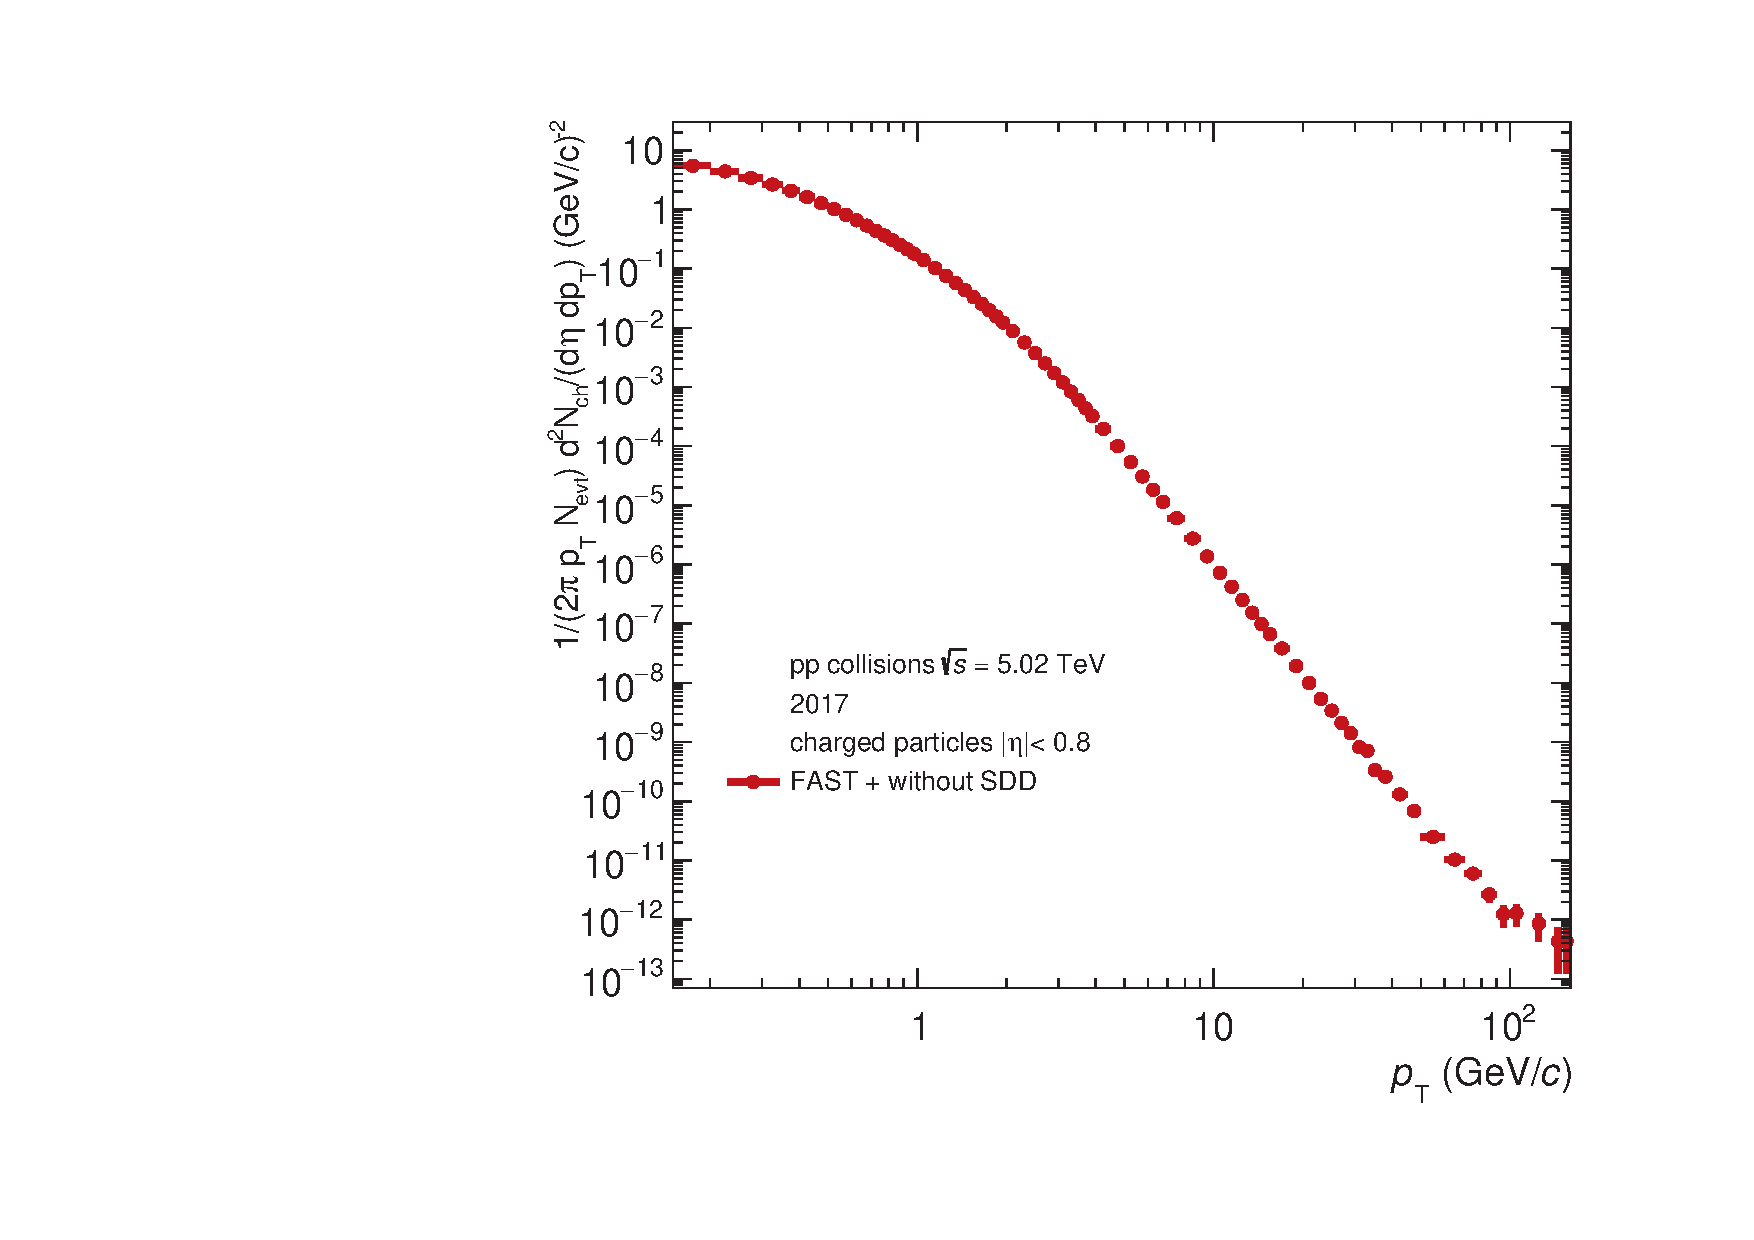
\includegraphics[width=12.5cm]{Plots/correctedSpectrum.pdf}  
\caption{Korrigierte Transversalimpulsverteilung geladener Teilchen in pp-Kollisionen bei $\sqrt{s} = 5.02$ TeV von 2017.}
\label{correctedSpectrum}
\end{figure}
\begin{figure}[H]
\centering
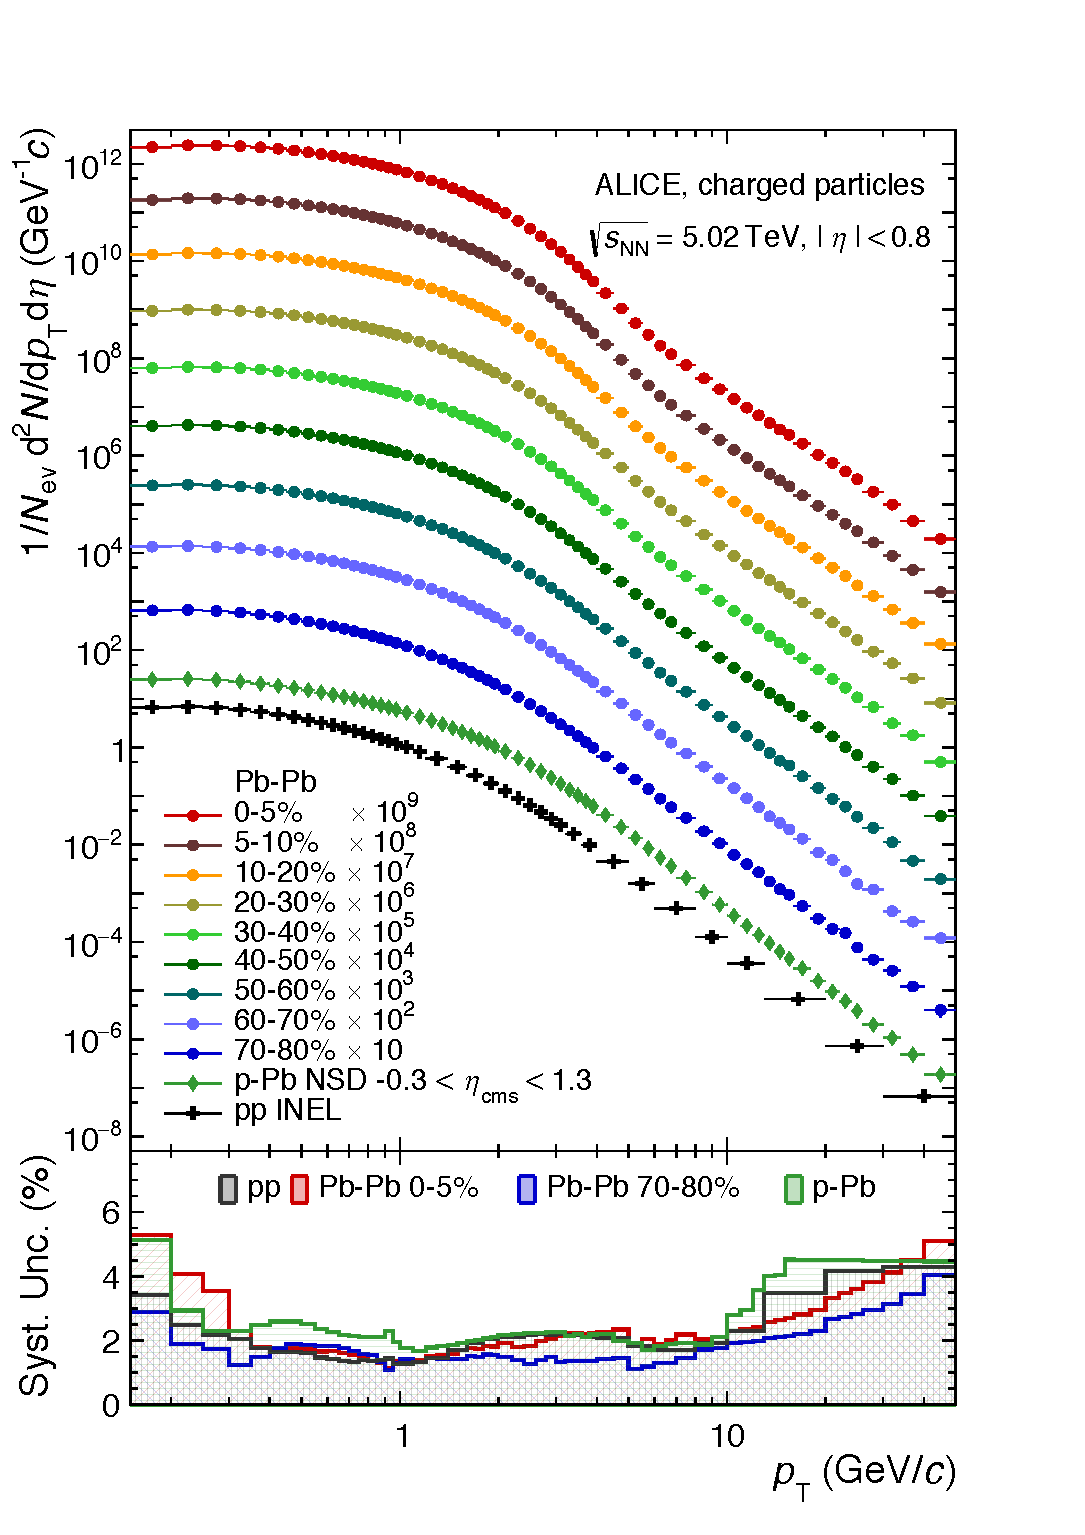
\includegraphics[width=9cm]{Plots/PublishedResults.pdf}  
\caption{Transversalimpulsverteilung geladener Teilchen in Pb-Pb-Kollisionen in neun Zentralitätsbereichen sowie in p-Pb- und pp-Kollisionen bei $\sqrt{s} = 5.02$ TeV von 2015 \cite{Acharya:2018qsh}.}
\label{PublishedResults}
\end{figure}
\section{Systematische Unsicherheiten} 
Der vorliegende Abschnitt dient dem Zweck, die Quellen der systematischen Unsicherheiten der hier präsentierte Analyse zu beschreiben und ferner diese Unsicherheiten auszuwerten. Die verschiedenen Quellen dafür wirken unabhängig voneinander. Aus diesem Grund ergibt sich der gesamte Wert systematischer Unsicherheiten aus der quadratischen Summe der einzelnen Beiträge:
\begin{equation}
\sigma_{sys, ges} = \sqrt{\sum_{i}{\sigma_{sys, i}}^2}
\end{equation}
Dieser gesamte Wert beträgt für die vorgestellte Analyse $\sigma_{sys, ges} = 4.53$ \%. Wie die einzelnen Beiträge berechnet wurden und welche Quellen berücksichtigt wurden, wird im Folgenden ausführlich behandelt.
\subsection{Auswahlkriterien}
%\vspace{-1em}
\begin{table}[H]
\centering
\begin{tabular}{|l c c c|}
\hline
 \multicolumn{1}{c}{\textbf{Spurselektion}} & \multicolumn{1}{c}{\textbf{Nominalwert}} & \multicolumn{2}{c|}{\textbf{Variationen}}\\
\hline
\hline
 max. $\mathrm{DCA}_{z}$ & $2$ cm & $1$ cm & $5$ cm\\
\rowcolor{mygray}   & & &\\

max. $\mathrm{DCA}_{xy}$ & $7\sigma$ & $4\sigma$ & $10\sigma$\\
  & & &\\
 
\rowcolor{mygray}  Auftreffen des Teilchens & benötigt  & \multicolumn{2}{c|}{nicht benötigt}\\
\rowcolor{mygray}  auf das SPD & & \multicolumn{2}{c|}{ }\\


max. Anteil von Spuren, die & $0.4$ & $0.2$ & $1.0$\\
  TPC-Cluster teilen & & &\\


\rowcolor{mygray}  max. Verhältnis von durchgequerten & $0.8$ & $0.7$ & $0.9$\\
\rowcolor{mygray}     Reihen zu auffindbaren Clustern & & &\\

 geometrische Länge der Spur & $130$ & $120$ & $140$\\
  & & &\\

\rowcolor{mygray}  geometrische Länge des & $3$ cm & $2$ cm & $4$ cm\\
\rowcolor{mygray}   TPC-Ausschlussgebiets & & &\\

 max. $\chi^2$ per TPC-Cluster & $2.5$ & $1.7$ & $3.4$\\
 & & & \\

\rowcolor{mygray}  max. $\chi^2$ per ITS-Cluster  & $36$ & $25$ & $49$\\
\rowcolor{mygray}  & & &\\

 max. $\chi^2$ der in TPC  & $36$ & $25$ & $49$\\
 begrenzter Spur vs. globale Spur & & &\\
\hline
\end{tabular}
\caption{Zusammenfassung der durchgeführten Variationen der Spurselektionen.}
\label{tab:CutsVariation}
\end{table}
\vspace{-1em}
Die Kriterien für die Spurselektion stellen eine zu betrachtende Quelle systematischer Unsicherheit dar. Jedes Auswahlkriterium trägt zur systematischen Unsicherheit vollkommen unabhängig von den anderen Kriterien bei.\\
Um die Beiträge der Spurselektionen auszurechnen, werden zuerst die in der Tabelle \ref{tab:Cuts} vorhandenen Werte einzeln innerhalb eines physikalisch sinnvollen Bereich variiert, wie die Tabelle \ref{tab:CutsVariation} zeigt. Anschließend wird bei jeder Variation das entsprechende korrigierte $p_{\mathrm{T}}$-Spektrum berechnet, ohne die anderen Selektionen zu modifizieren. Im Anschluss werden die Unterschiede im korrigierten $p_{\mathrm{T}}$-Spektrum mit dem nominellen $p_{\mathrm{T}}$-Spektrum herausgearbeitet. Diese Unterschiede werden als systematische Unsicherheit bei dieser Selektion betrachtet. Bei jedem $p_{\mathrm{T}}$-Intervall wird ferner das quadratische Mittel aller Spurselektionen berechnet. Auf diese Weise erhält man die Verteilung der kombinierten systematischen Unsicherheit. In der Abbildung \ref{SysUncTrack} wird der Beitrag der verschiedenen Spurselektionen an die systematischen Unsicherheiten sowie die sich daraus ergebende kombinierte Verteilung in Abhängigkeit vom Transversalimpuls $p_{\mathrm{T}}$ dargestellt. In der Tabelle \ref{tab:SysUnsich} findet man zusätzlich eine Übersicht der Maximalwerte dieser Beiträge in Prozent. Das Maximum der kombinierten Kurve wird als Referenzwert zum Beitrag der Spurselektion an die systematische Unsicherheit verwendet.
\begin{figure}[tb!]
\centering
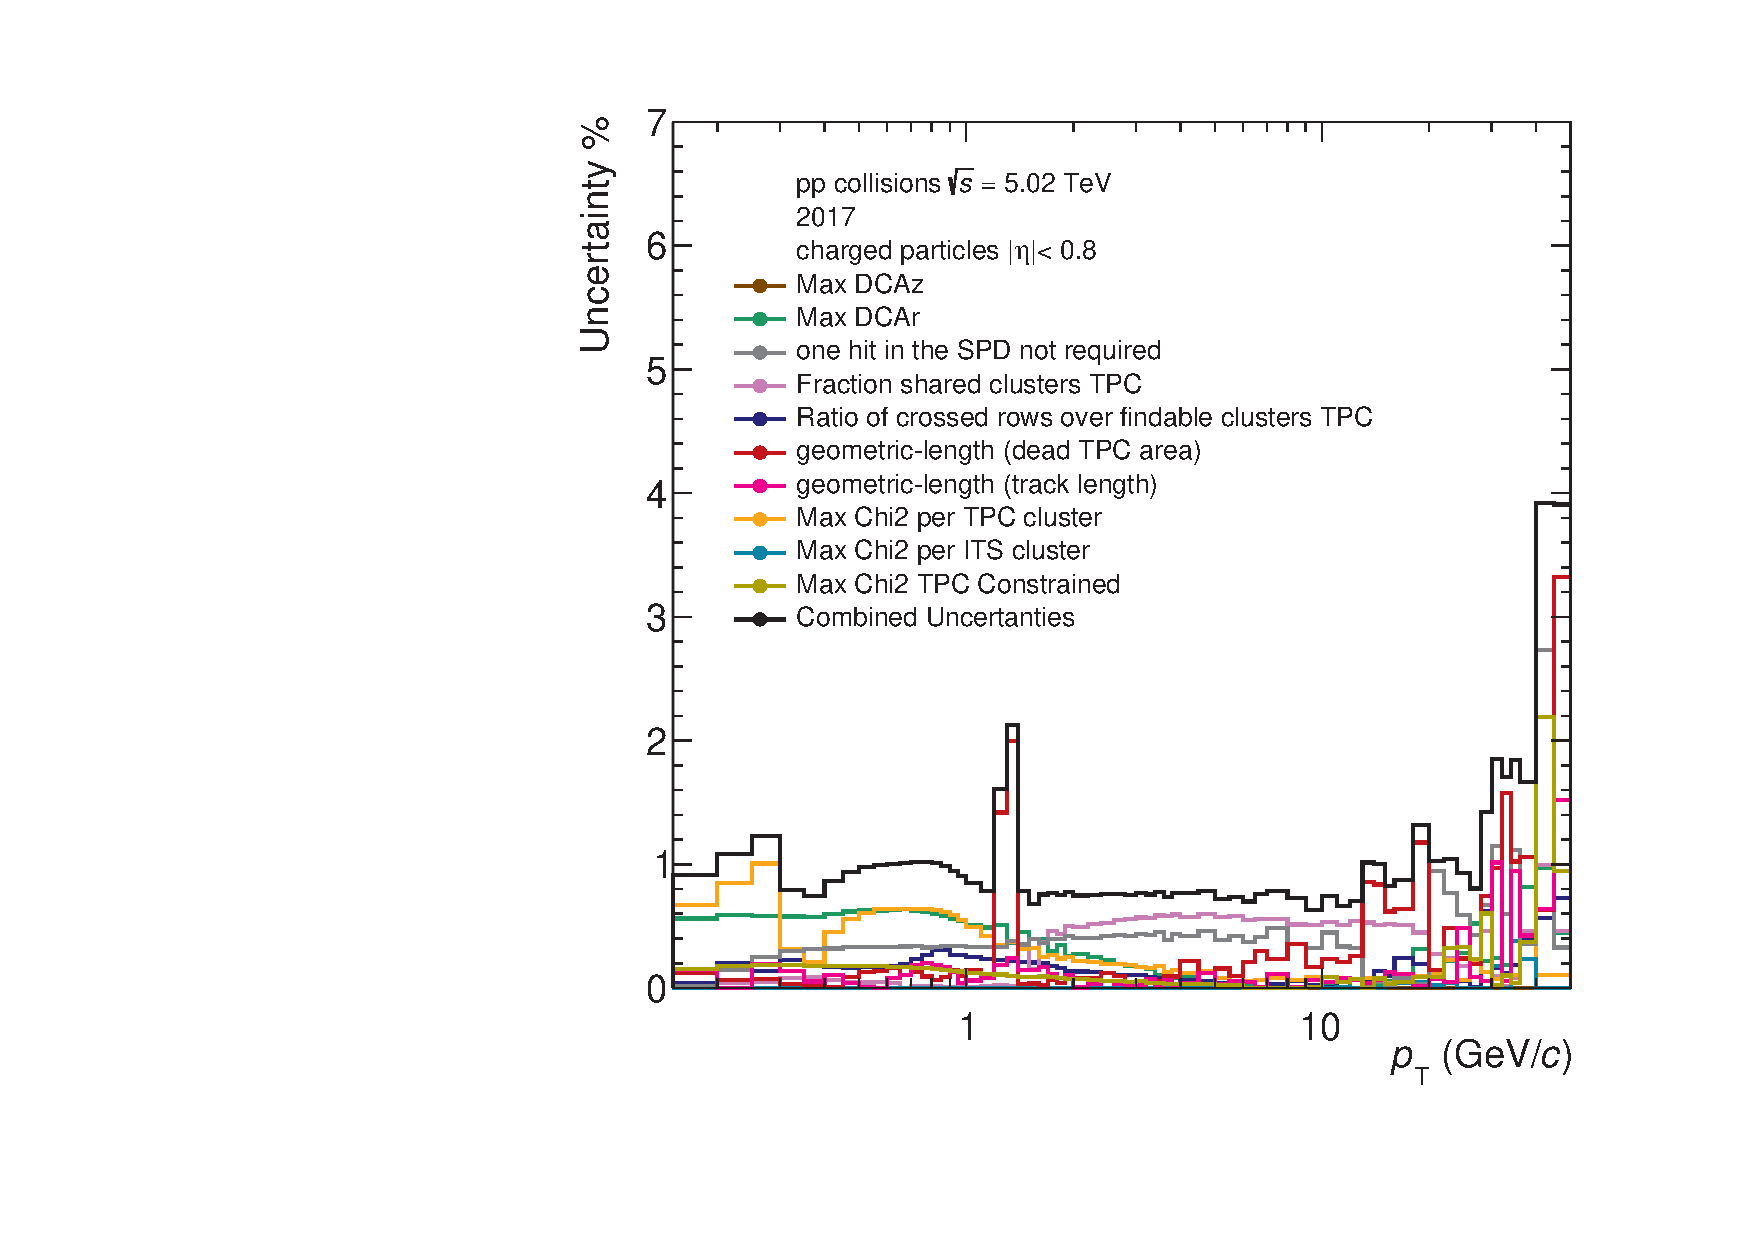
\includegraphics[width=12.5cm]{Plots/SySUncTrack.pdf}  
\caption{Beiträge jeder Spurselektion der Analyse an die systematische Unisicheheit.}
\label{SysUncTrack}
\end{figure}
\begin{table}[H]
\centering
\begin{tabular}{|c c|}
\hline
\textbf{Id} & \textbf{Unsicherheit in $\%$}\\
\hline
\hline
\rowcolor{mygray} 1 & vernachlässigbar\\
		  2 & $0.97$\\
\rowcolor{mygray} 3 & $2.73$\\
		  4 & $0.94$\\
\rowcolor{mygray} 5 & $0.72$\\
		  6 & $1.52$\\
\rowcolor{mygray} 7 & $3.32$\\
		  8 & $1.00$\\
\rowcolor{mygray} 9 & $0.38$\\
		  10 & $2.19$\\
\hline
\hline
\rowcolor{mygray} \textbf{Gesamt} & $3.92$\\
\hline
\end{tabular}
\caption{Maximale Prozentwerte der systematischen Unsicherheiten jeder Spurselektion. Der Wert der kombinierten systematischen Unsicherheit wird als Gesamtbeitrag der Spurselektion benutzt.}
\label{tab:SysUnsich}
\end{table}
\subsection{\textit{Matching efficiency}}
\vspace{-1em}
\begin{table}[H]
\centering
\begin{tabular}{|c c|}
\hline
\textbf{$p_{\mathrm{T}}$-Intervall ($\mathrm{GeV}/c$)} & \textbf{Unsicherheit in $\%$}\\
\hline
\hline
\rowcolor{mygray} $0.8 - 1.0$ & $1.01$\\
		  $1.0 - 2.0$ & $2.00$\\
\rowcolor{mygray} $2.0 - 3.0$ & $2.66$\\
		  $3.0 - 4.0$ & $2.41$\\
\rowcolor{mygray} $4.0 - 6.0$ & $2.17$\\
		  $6.0 - 8.0$ & $2.09$\\
\rowcolor{mygray} $8.0 - 15.0$ & $2.28$\\
\hline
\hline
			 \textbf{Gesamt} & $2.28$\\
\hline
\end{tabular}
\caption{Systematische Unsicherheiten in $\%$ im Bezug auf die \textit{matching efficiency}. Dabei sind die ersten sieben $p_{\mathrm{T}}$-Intervalle dargestellt.}
\label{tab:MatchingEff}
\end{table}
Die Monte-Carlo-Simulationen versuchen, unter anderem das Verhalten der Detektoren unter bestimmten Bedingungen vorherzusagen. Trotzdem ist ihre Fähigkeit dafür limitiert. Da nicht alle Detektoreffekte berücksichtigt werden können, führt die Berechnung der Nachweiseffizienz, welche mithilfe von Monte-Carlo-Simulationen bestimmt wird, zu einer systematischen Unsicherheit.\\
Zu ihrer Abschätzung ermittelt man die Differenz zwischen den beiden Nachweis\-effizienzen, die aus den gemessenen Daten und den Monte-Carlo-Simulationen stammen. Um dies zu erreichen, evaluiert man in Daten und in den Monte-Carlo-Simulationen, in welchem Umfang die Spuren, die in der TPC gemessen wurden, mit der Information, die das ITS anbietet, übereinstimmt. Die Variable, die diese Übereinstimmung charakterisiert, heißt \textit{matching efficiency} und wird aus dem Verhältnis von der Anzahl von Spuren, die lediglich mit der TPC gefittet wurden, zur Anzahl globaler Spuren, welche mit dem gesamten Detektorsystem TPC-ITS erhalten wurden, berechnet. Dabei wird die Spurselektion leicht angepasst, damit die Kriterien für die Selektion primärer Spuren weniger streng werden.\\
Aufgrund der schon erwähnten begrenzten Kapazität der Monte-Carlo-Simulationen zeigt die \textit{matching efficiency} der Daten eine geringe, aber relevante Diskrepanz von der Monte-Carlo-Simulationen. Die Subtraktion von beiden Werten stellt die gesuchte systematische Unsicherheit dar. In der Tabelle \ref{tab:MatchingEff} kann man die zum untersuchten Datensatz gehörenden Unsicherheiten nachschlagen \cite{DataPG}. Die Untersuchung erfolgte nur für die ersten sieben $p_{\mathrm{T}}$-Intervalle, denn dies reicht, um das Auswerten vorzunehmen. Der Maximalwert wird als Beitrag an die systematische Unsicherheit benutzt.

\chapter{Zusammenfassung}
Die in der vorliegenden Arbeit vorgestellte Analyse untersucht die Produktionsrate primärer geladener Teilchen in Proton-Proton-Kollisionen bei einer Schwerpunktsenergie von $\sqrt{s} = 5.02$ TeV im ALICE-Experiment. Dabei wird das $p_{\mathrm{T}}$-Spektrum dieser Teilchen bestimmt. Die Messung der verwendeten Kollisionen wurde im Jahr 2017 vorgenommen. In diesem Zusammenhang wurden zwei verschiedenen Einstellungen des Detektorsystems angewendet: \textit{CENT} und \textit{FAST}. Bei \textit{CENT} wurden alle Detektoren bei der Datennahme eingesetzt, während die SDD-Schichten bei \textit{FAST} zur Gewinnung höherer Anzahl von Ereignissen nicht verwendet wurden. Die Ereignisse von \textit{CENT} wurden ferner ohne den SDD zum Zwecke des Vergleichs rekonstruiert. In dieser Arbeit wird auf die Maximalanzahl von Ereignissen zurückgegriffen, indem man zeigt, dass sich \textit{FAST} und \textit{CENT} ohne SDD so ähneln, dass sie kombiniert betrachtet werden können.\\
Um die Qualität der analysierten Ereignisse und der primärer geladenen Teilchen zu gewährleisten, werden unterschiedliche Selektionskriterien verlangt, die die nicht-physikalisch relevanten gemessenen Daten von der Analyse ausschließen. Im Resultat ergibt sich ein unkorrigiertes $p_{\mathrm{T}}$-Spektrum, das eine Detektor abhängige Produktionsrate geladener Teilchen als Funktion des Transversalimpulses beschreibt.\\
Zur Aufhebung des Einflusses der Detektoren auf die Analyse werden verschiedene Korrekturen mithilfe von Monte-Carlo-Simulationen entwickelt. Die Nachweis\-effizienz stellt beispielsweise die Nachweiswahrscheinlichkeit der Detektoren für die Messung der Teilchen dar. Das $p_{\mathrm{T}}$-Spektrum muss dahingehend korrigiert werden. Zusätzlich wird die Kontamination durch Sekundärteilchen auch berechnet und die gemessenen Daten korrigiert werden. Die Messung der Krümmung der Spuren erfolgt außerdem mit einer konkreten Ungenauigkeit. Der Transversalimpuls geladener Teilchen wird anhand dieser Krümmung bestimmt und dies impliziert ebenfalls die Existenz einer Abweichung der gemessenen Daten, deren Auswirkung entsprechend abgeschätzt wird. Schließlich stellt die Normierung des $p_{\mathrm{T}}$-Spektrums auf die Anzahl unelastischer Kollisionen den letzten Schritt in diese Richtung dar.\\
Nach erfolgreicher Anwendung der Korrekturen wird das resultierende $p_{\mathrm{T}}$-Spektrum evaluiert und mit vergangenen Ergebnissen einer analogen Analyse vom 2015 verglichen. Es stellt sich heraus, dass die vorgestellte Analyse Fortschritte im Bezug auf die Reichweite und die Granularität des $p_{\mathrm{T}}$-Spektrums aufweist und eine bessere Referenzmessung zur Beschreibung von Schwerionenkollisionen darstellt. Die Verwendung dieser Arbeit als eine solche Referenzmessung eröffnet vielfältige Möglichkeiten für spätere Analysen von Schwerionenkollisionen und ermöglicht ein präziseres und damit besseres Verständnis der Physik des Quark-Gluon-Plasmas.

\cleardoublepage
\addcontentsline{toc}{chapter}{Literaturverzeichnis}
\bibliographystyle{alpha}
\bibliography{mybib}



\chapter*{Danksagung}
\pagenumbering{gobble}
Zuallererst möchte ich mich herzlich bei Prof. Dr. Henner Büsching bedanken, der es mir ermöglicht hat, meine Bachelorarbeit in seiner Arbeitsgruppe zu schreiben. Außerdem danke ich ihm dafür, dass er immer ein offenes Ohr für meine Fragen hatte, welche manchmal auch außerhalb der Arbeit waren.\\
Zusätzlich gilt mein Dank Prof. Dr. Harald Appelshäuser, der sich als Zweitgutachter zur Verfügung gestellt hat.\\
Zudem möchte ich mich besonders bei Patrick Huhn für die Betreuung dieser Arbeit bedanken. Ohne seine zahlreichen Hilfestellungen und die anregenden Diskussionen mit ihm wäre die Arbeit nicht zustande gekommen. In diesem Zusammenhang danke ich ebenfalls speziell Mario Krüger, der geduldig meine Fragen beantwortet hat.\\
Weiterhin gilt mein Dank der gesamten Frankfurter Arbeitsgruppe für die freundliche Aufnahme und für all die schönen Momente.\\
Schließlich gilt mein besonderer Dank meinen Eltern und meinen Geschwistern, die mir mein Studium ermöglicht und mich in all meinen Entscheidungen unterstützt haben.
\nocite{alice}
\chapter*{Eigenständigkeitserklärung}
Hiermit erkläre ich, dass ich die Bachelorarbeit selbstständig und ohne Benutzung anderer als der angegebenen Quellen und Hilfsmittel verfasst habe. Alle Stellen der Arbeit, die wörtlich oder sinngemäß aus Veröffentlichungen oder aus anderen fremden Texten entnommen wurden, sind von mir als solche kenntlich gemacht worden. Ferner erkläre ich, dass die Arbeit nicht -auch nicht auszugsweise- für eine andere Prüfung verwendet wurde.\\ \\ \\ \\ \\ 
\hspace*{1cm}  Frankfurt am Main, 18.02.2019   \hspace*{2cm}   Youssef El Mard Bouziani

\chapter*{}
\end{document}
